% Author: Sandy Burden, Version 1
% ----------------------------------------------------------------
% NIASRA Beamer template for Slides *******************************
% ----------------------------------------------------------------
\documentclass{beamer}
%\documentclass[handout]{beamer}
%\pgfpagesuselayout{4 on 1}[a4paper, border shrink=5mm, landscape]

\usepackage{color}
\usepackage{pgfpages}
\usepackage{graphicx}
\usepackage[utf8]{inputenc}
\usepackage[T1]{fontenc}
\usepackage{amsmath,amsthm, amssymb}
\usepackage{amsfonts}
\usepackage{natbib}
\usepackage{bm}
\usepackage{setspace}


\pdfmapfile{+sansmathaccent.map}

\hfuzz5pt % Don't bother to report over-full boxes < 5pt
\vfuzz5pt % Don't bother to report over-full boxes < 5pt
\setlength{\parskip}{3mm}
\usetheme{NIASRA}

% Include secheader option if you want section headers at top of slide.  Can get wide...
%\usetheme[secheader]{NIASRA}

\newcommand{\Yt}{\widetilde{Y}}
\newcommand{\Deltab} {\boldsymbol{\Delta}}
\newcommand{\intd} {\mathrm{d}}
\newcommand{\Bmat} {\textbf{B}}
\newcommand{\Dmat} {\textbf{D}}
\newcommand{\Qmat} {\textbf{Q}}
\newcommand{\Cmat} {\textbf{C}}
\newcommand{\cmat} {\textbf{c}}
\newcommand{\Imat} {\textbf{I}}
\newcommand{\bvec} {\textbf{b}}
\newcommand{\svec} {\textbf{s}}
\newcommand{\uvec} {\textbf{u}}
\newcommand{\omegab} {\boldsymbol {\omega}}
\newcommand{\s}{\mathbf{s}}
\newcommand{\h}{\mathbf{h}}
\renewcommand{\b}{\mathbf{b}}
\newcommand{\z}{\mathbf{z}}
\renewcommand{\v}{\mathbf{v}}
\renewcommand{\u}{\mathbf{u}}
\newcommand{\w}{\mathbf{w}}
\renewcommand{\d}{\mathrm{d}}
\newcommand{\Z}{\mathbf{Z}}
\newcommand{\x}{\mathbf{x}}
\newcommand{\Y}{\mathbf{Y}}
\newcommand{\Yvec}{\mathbf{Y}}
\newcommand{\Zvec}{\mathbf{Z}}
\newcommand{\epsilonb}{\boldsymbol{\varepsilon}}
\newcommand{\bI}{\mathbf{I}}
\newcommand{\bB}{\mathbf{B}}
\newcommand{\bbeta}{\boldsymbol{\beta}}
\newcommand{\thetab}{\boldsymbol{\theta}}
\newcommand{\bzero}{\boldsymbol{0}}
\newcommand{\bSigma}{\bm{\Sigma}}
\newcommand{\E}{E}
\newcommand{\cov}{\mathrm{cov}}
\newcommand{\var}{\mathrm{var}}
\newcommand{\tr}{\mathrm{tr}}
\newcommand{\diag}{\mathrm{diag}}
\newcommand{\vect}{\mathrm{vec}}
\newcommand{\Gau}{\mathrm{Gau}}
\newcommand{\RR}{\mathbb{R}}
\newcommand{\varthetab} {{\boldsymbol{\vartheta}}}
\newcommand{\Dist}{\mathrm{Dist}}
\newcommand{\ff} {\textit{ff}}

\newcommand{\red}{\textcolor{red}}%
\newcommand{\blue}{\textcolor{blue}}

\bibliographystyle{apa}

 \title[Atmospheric trace gas inversions]{Bivariate spatio-temporal statistical models for atmospheric trace gas inversions}
 \subtitle{-- joint work with Noel Cressie, Anita Ganesan and Matt Rigby --} %Not required if you dont want it
 \author[A. Zammit-Mangion]{Andrew Zammit-Mangion} %
  \institute[]{National Institute for Applied Statistics Research Australia \\  University of Wollongong \\ \vspace{0.4in} 
\includegraphics[height=1cm]{NiasraUowLonghand}} % Substitute date of presentation or include todays date instead.
\date{}
\begin{document}

\begin{frame}
\titlepage
\end{frame}

% The following slide provides a table of contents for the presentation.  Include or leave out as required.  Additional contents for individual sections can be included throughout the presentation using \tableofcontents[currentsection] or currentsubsection or hideallsubsections, subsubsectionstyle=hide etc.

\setstretch{1.5}

% \begin{frame}
% \frametitle{Outline}
%   \begin{minipage}{\textwidth}
%     \tableofcontents
%   \end{minipage}
% \end{frame}

% \frame{\frametitle{Outline}\tableofcontents}

\setstretch{1.1}


% \section{Introduction}

% \begin{frame}
% \sectionpage
% \end{frame}



% ###################

\begin{frame}
\frametitle{Introduction}

\begin{itemize}
\item {\bf Univariate} spatial/spatio-temporal model. \vfill

\item {\bf Multivariate} spatial/spatio-temporal model. \vfill
\begin{itemize}
    \item Two or more interacting variables. \vfill
    \item Improve prediction on one of the variates by observing the others: {\bf Cokriging}. \vfill
    \item Determine which variate caused the observed phenomenon: {\bf Source separation}, \citet{Zammit_2014,Zammit_2015b,Zammit_2015a}, Antarctica. \vfill
\end{itemize}\vfill
\end{itemize}

\end{frame}

% % ###################

% \begin{frame}
% \frametitle{Example 1: Ozone vs MaxT}

% \cite{RoyleBerliner1999}, Midwestern USA.

% \begin{center}
% 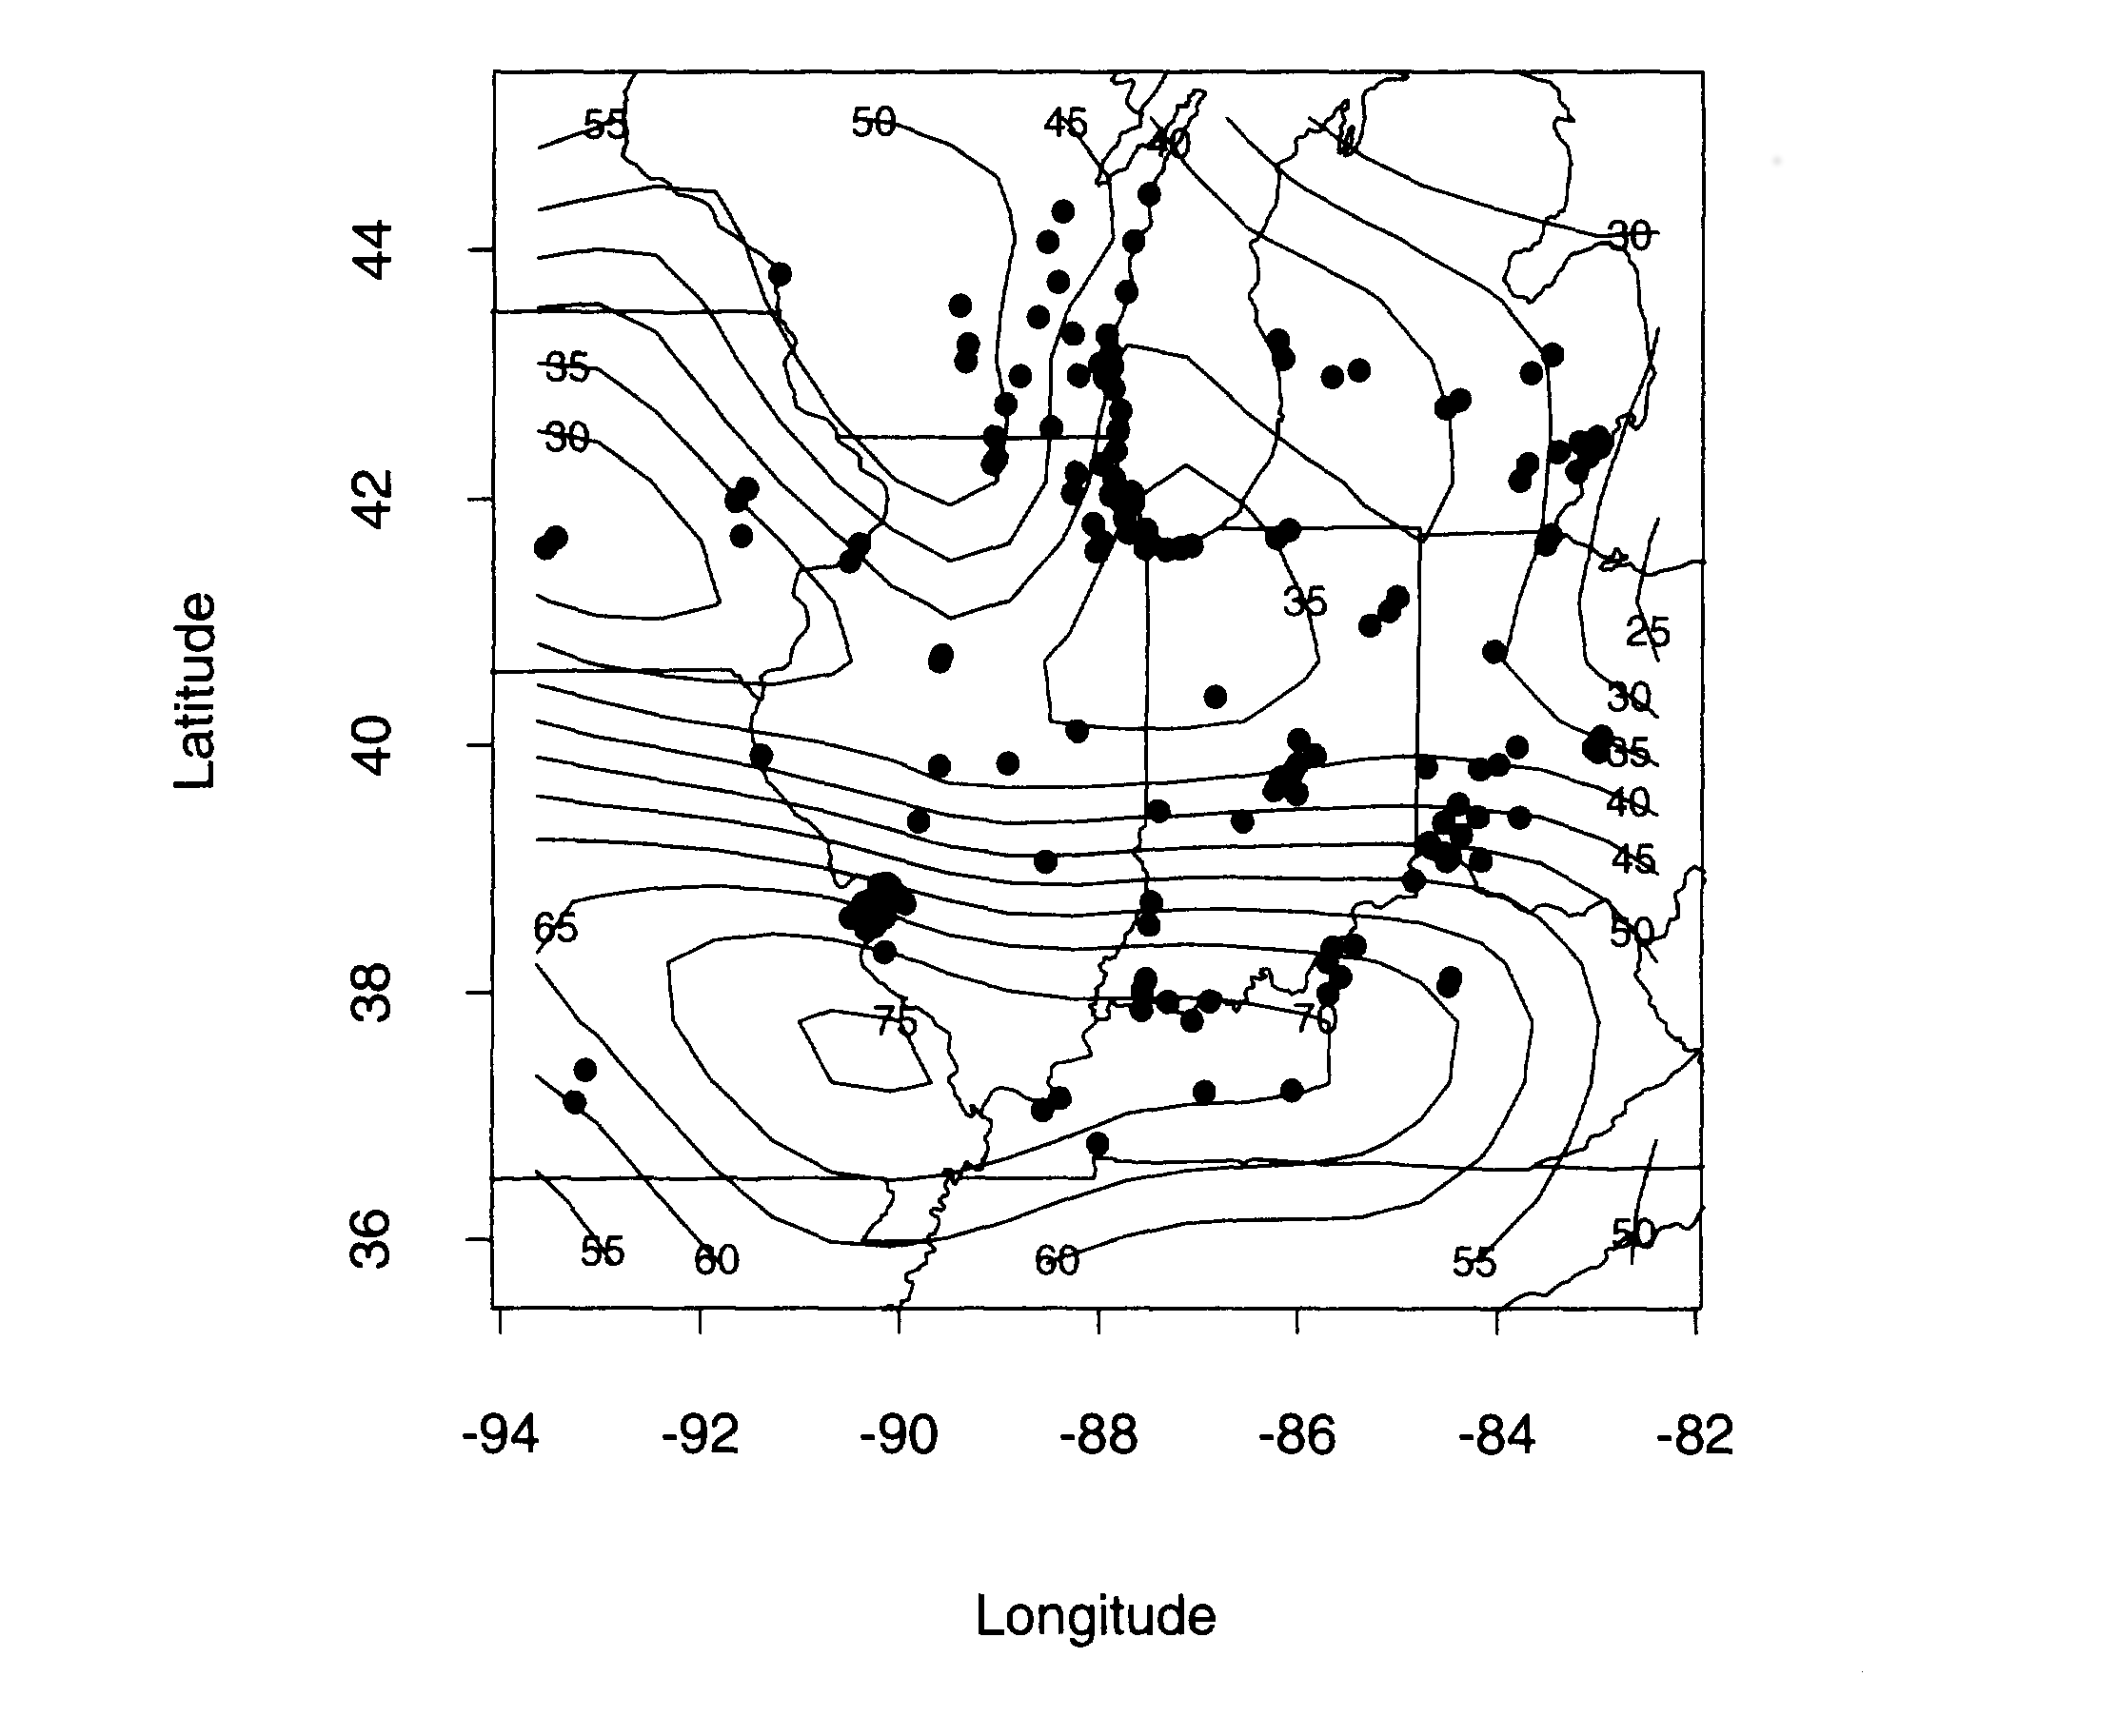
\includegraphics[width=2.5in]{./ozone.png}
% 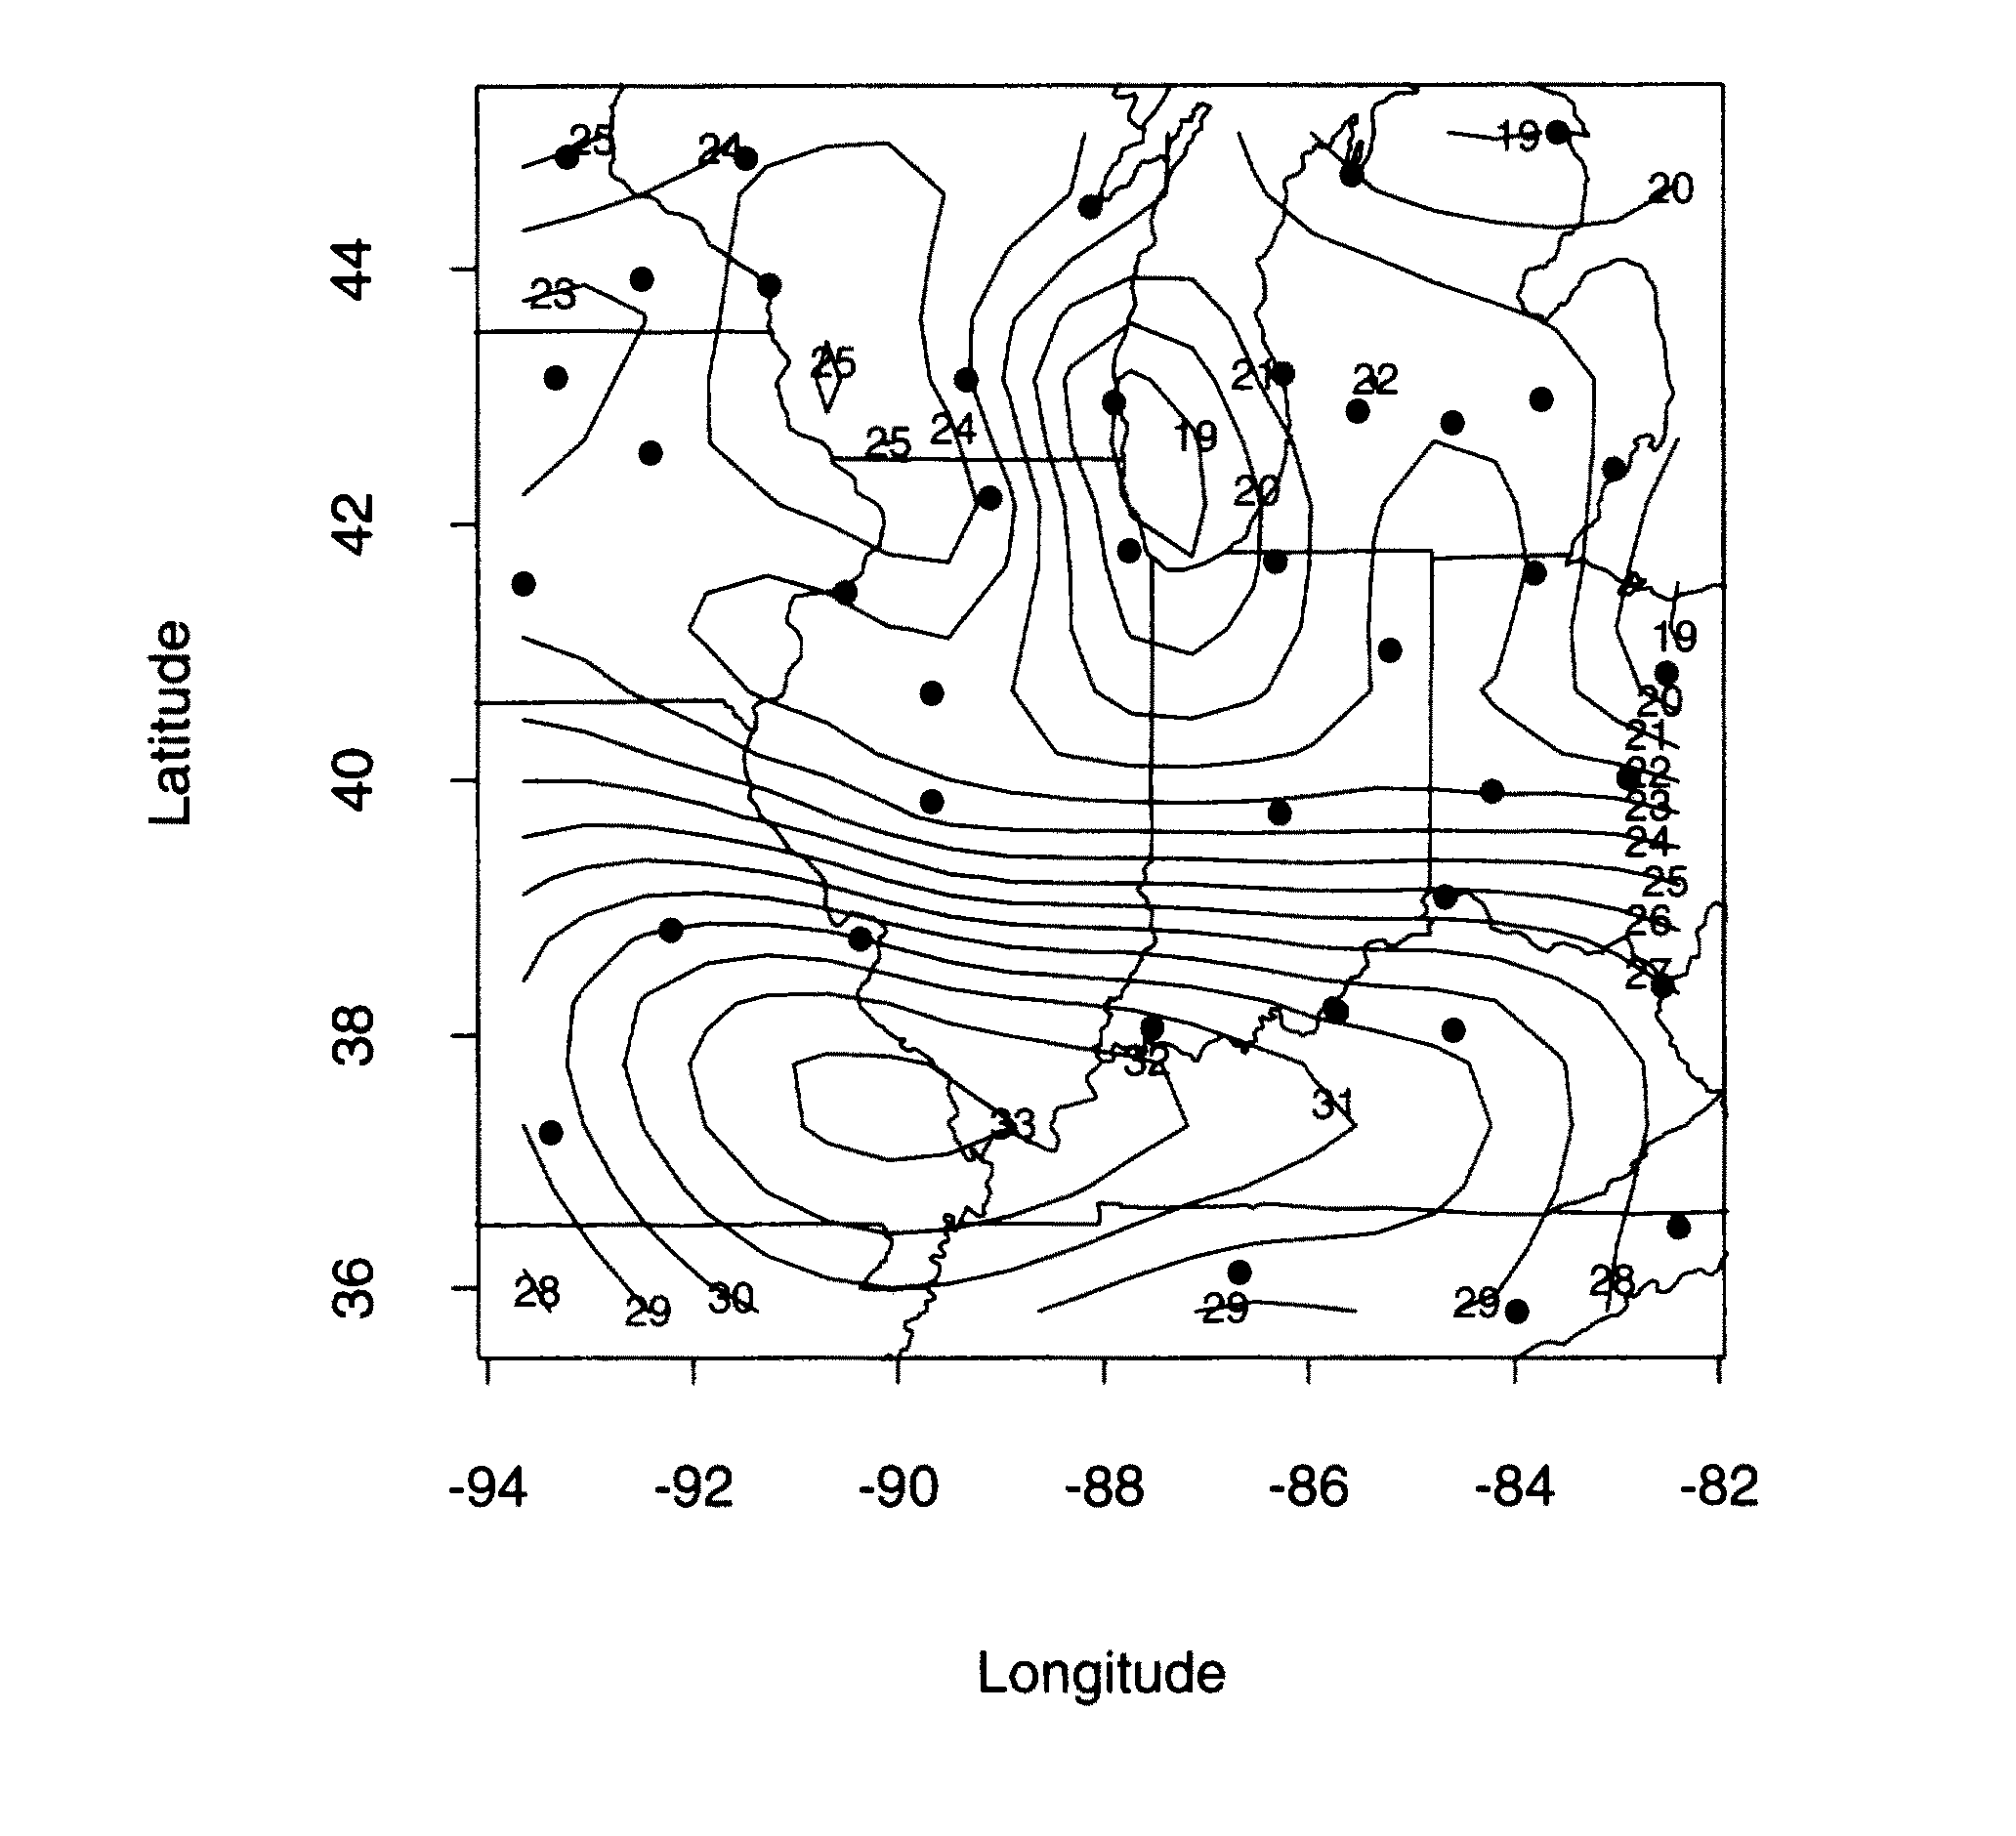
\includegraphics[width=2.3in]{./maxt.png}
% \end{center}
% \end{frame}

% % ###################

% \begin{frame}
% \frametitle{Example 2: Antarctica Mass Balance}

% 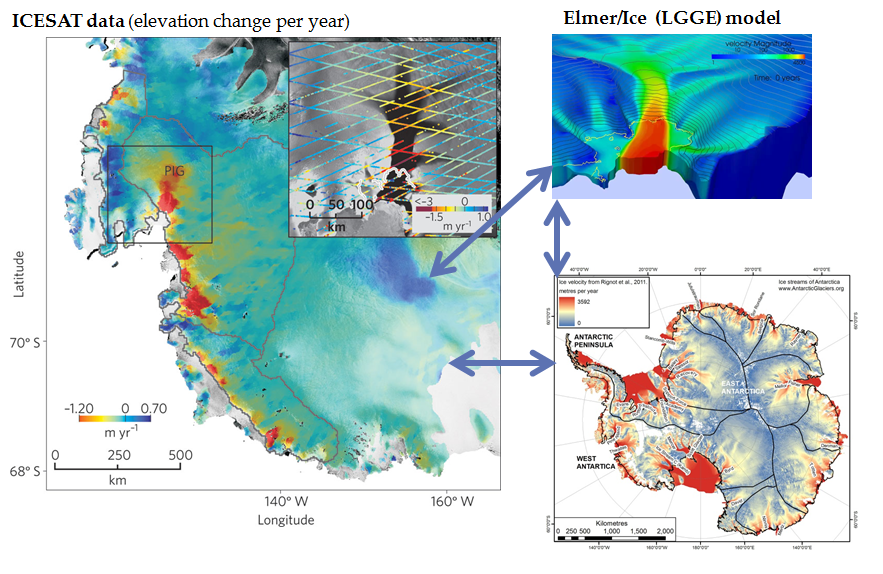
\includegraphics[width=4.5in]{./Antarctica.png}
% \end{frame}

% % ###################

% \begin{frame}
% \frametitle{Example 2: Antarctica Mass Balance}

% \begin{itemize}
% \item \citet{Zammit_2014,Zammit_2015b,Zammit_2015a}, Antarctica.
% \end{itemize}


% \begin{center}
% 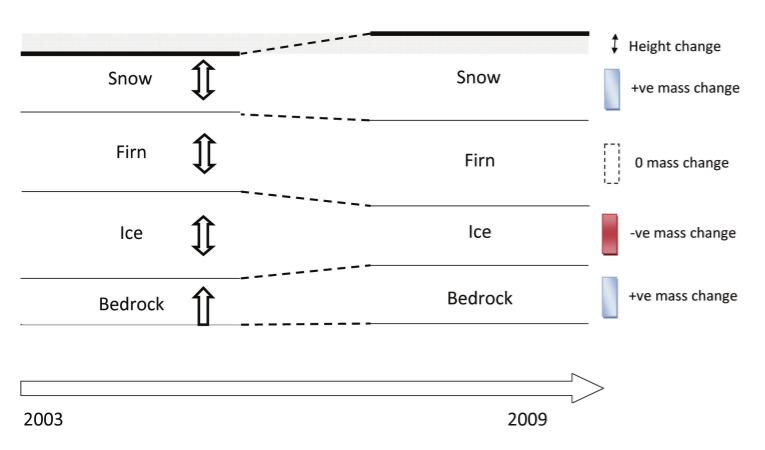
\includegraphics[width=4in]{./Obs.png}
% \end{center}

% \end{frame}

% % ###################



\section{Atmospheric trace-gas inversion}


% \begin{frame}
% \sectionpage
% \end{frame}

\begin{frame}
\frametitle{Atmospheric trace-gas inversion}

\begin{itemize}
\item $Y_1(\svec) \equiv Y_f(\svec)$ is methane flux per unit area -- we assume this is temporally invariant over a period of one month. \vfill
\item $Y_{2,t}(\svec) \equiv Y_{m,t}(\svec)$ is methane mole fraction (in ppm) and is spatio-temporally varying due to varying weather patterns etc. \vfill
%\item Only the mole fractions are observed. \vfill
\item {\bf Aim:} Infer the (spatial) emissions from observation of (spatio-temporal) mole fraction.\vfill
%\item Interaction function (SRR) $b_t(\svec,\uvec)$ is the influence of the emissions on the methane, affected by weather, pressure systems etc.\vfill
%\item Methane is a greenhouse gas which absorbs 100x more heat than CO$_2$.
\end{itemize}
\end{frame}

\begin{frame}
\frametitle{What is available?}

\begin{columns}[T]
\begin{column}{0.6\textwidth}
\small
  \begin{itemize}
  \item Methane emissions inventories, (e.g., the National Atmospheric Emissions Inventory (NAEI)).\vfill
  \item A Lagrangian Particle Dispersion Model (LPDM) is used to trace particles backwards in time and thus establish the flux-mole-fraction interaction function (SRR), $b_t(\svec,\uvec)$.\vfill
  \item The LPDM we use is the Met Office's National Atmospheric Modelling Environment (NAME).\vfill
  \item Data available at four measuring stations averaged over 2 h time periods.\vfill
  \end{itemize}
\end{column}
\hfill
\begin{column}{0.33\textwidth}

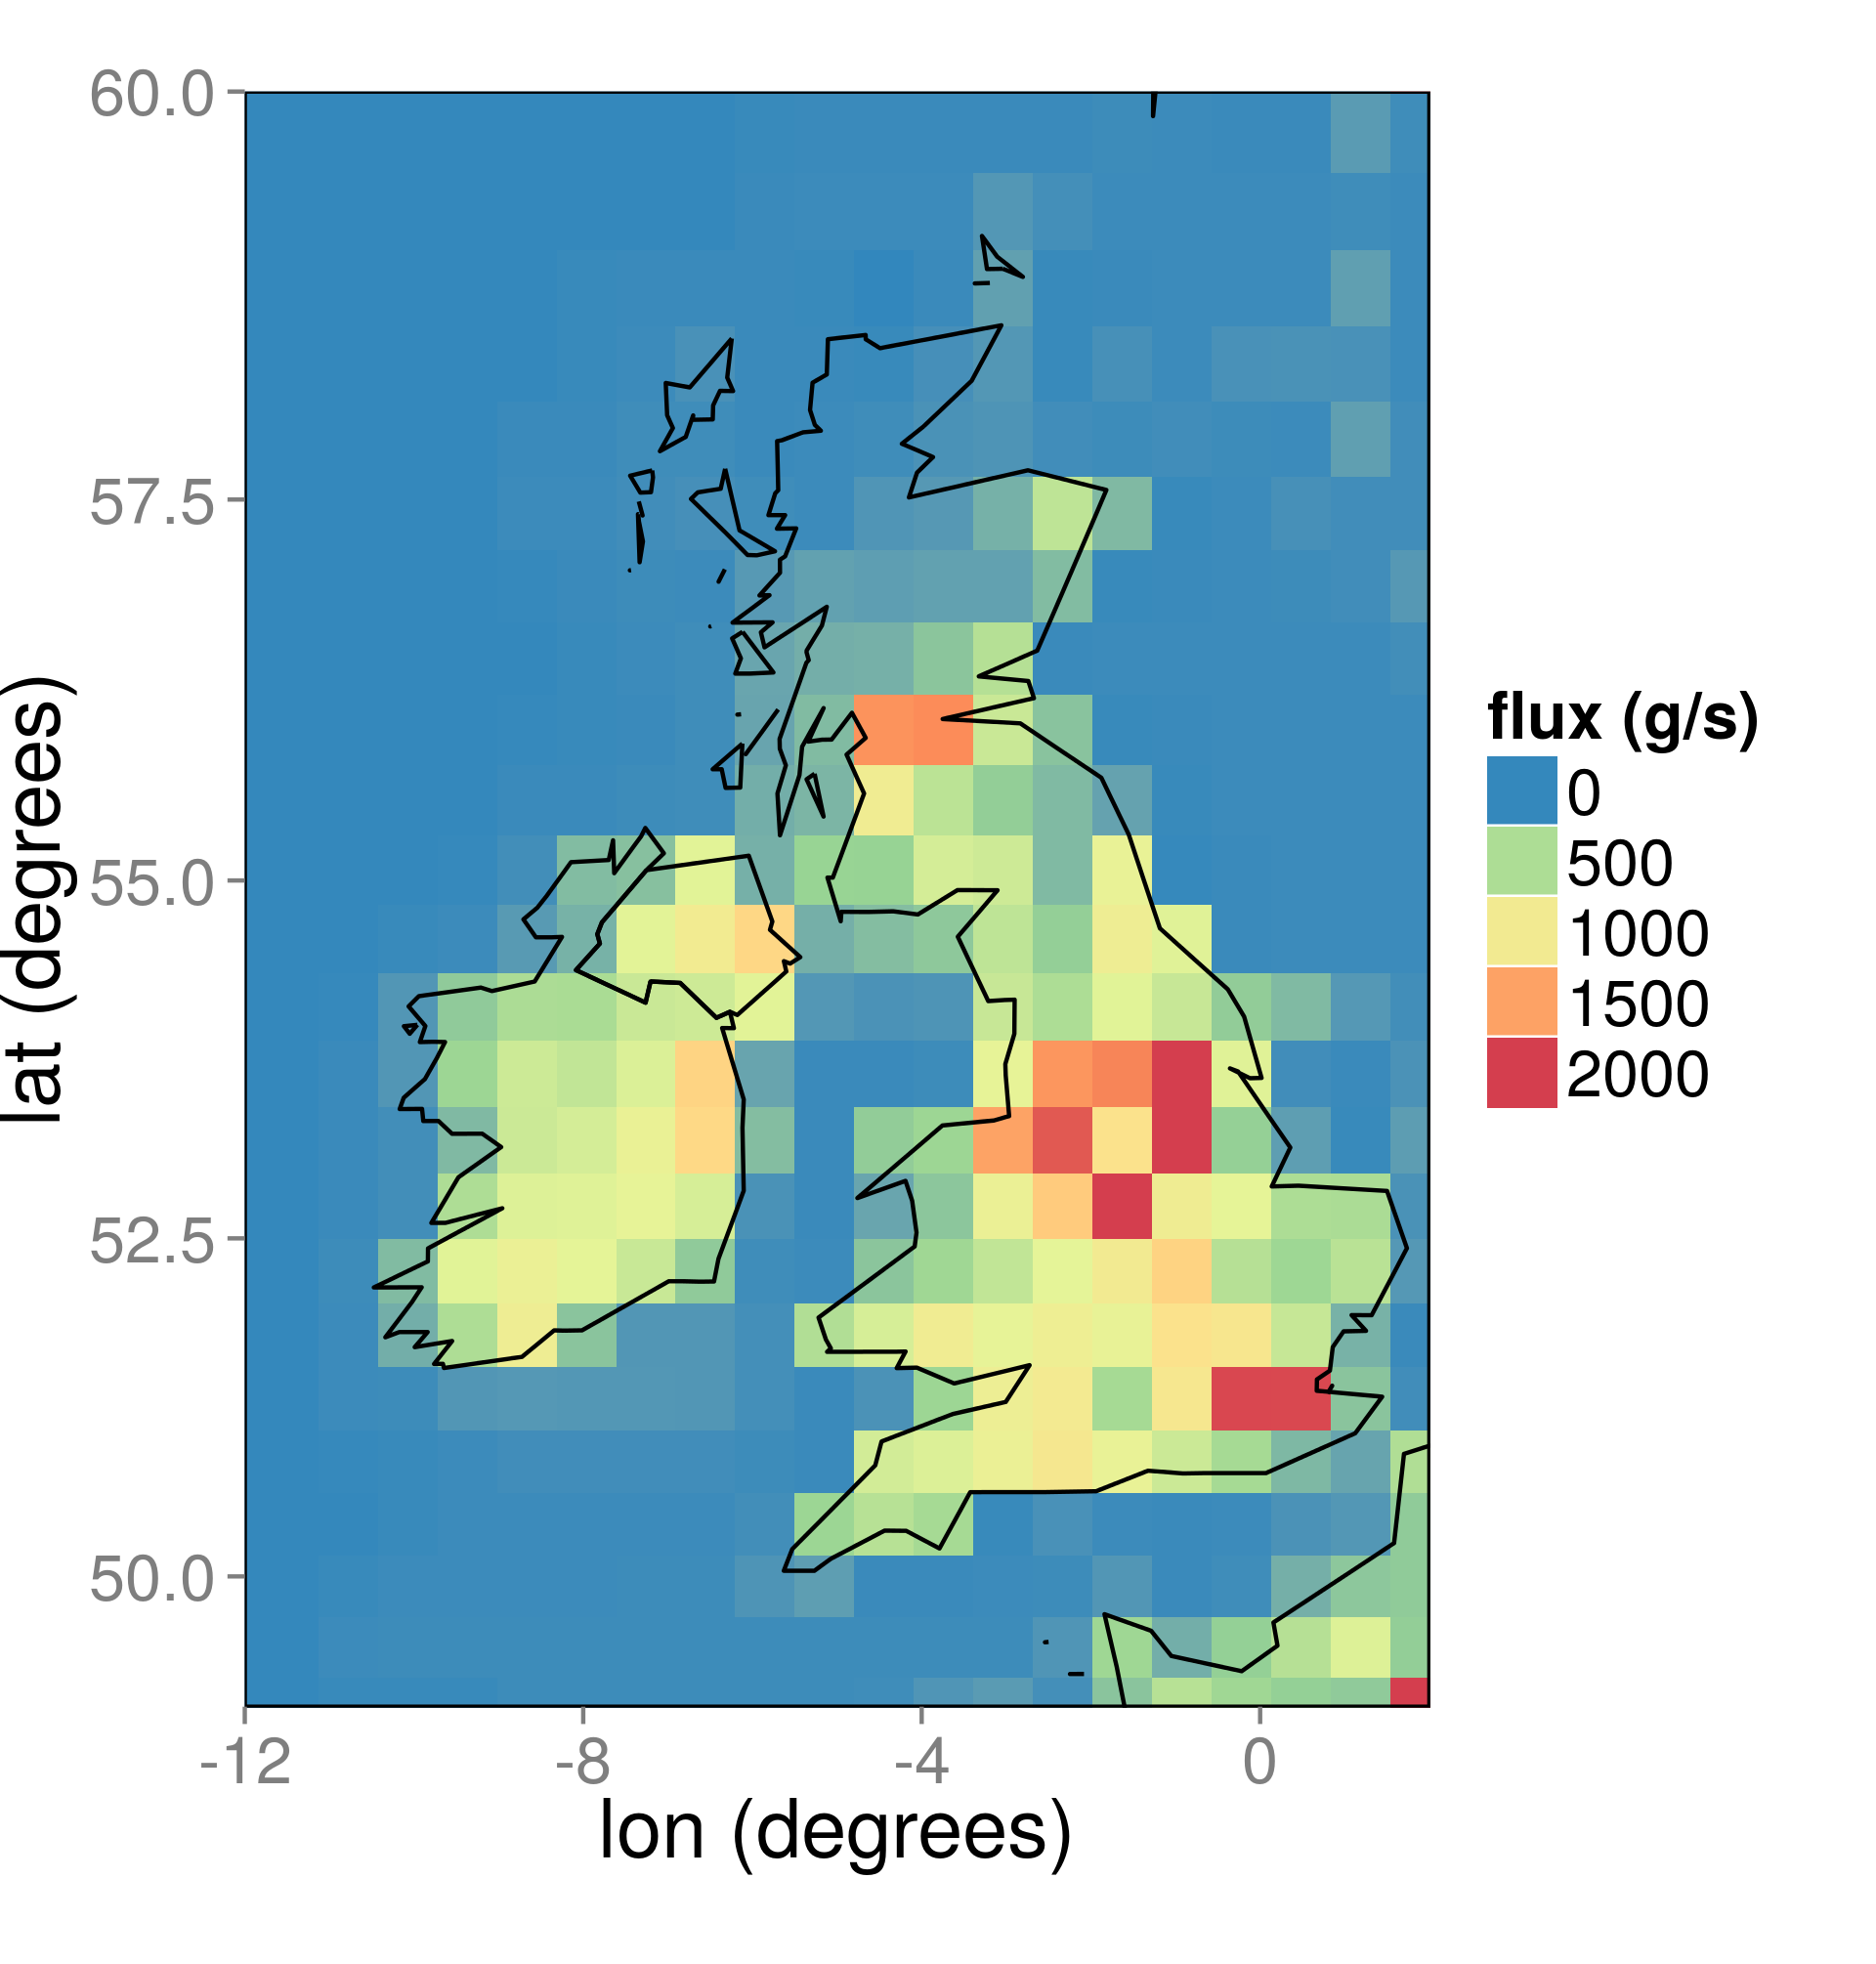
\includegraphics[width=1.4in]{NAEI.png} \\
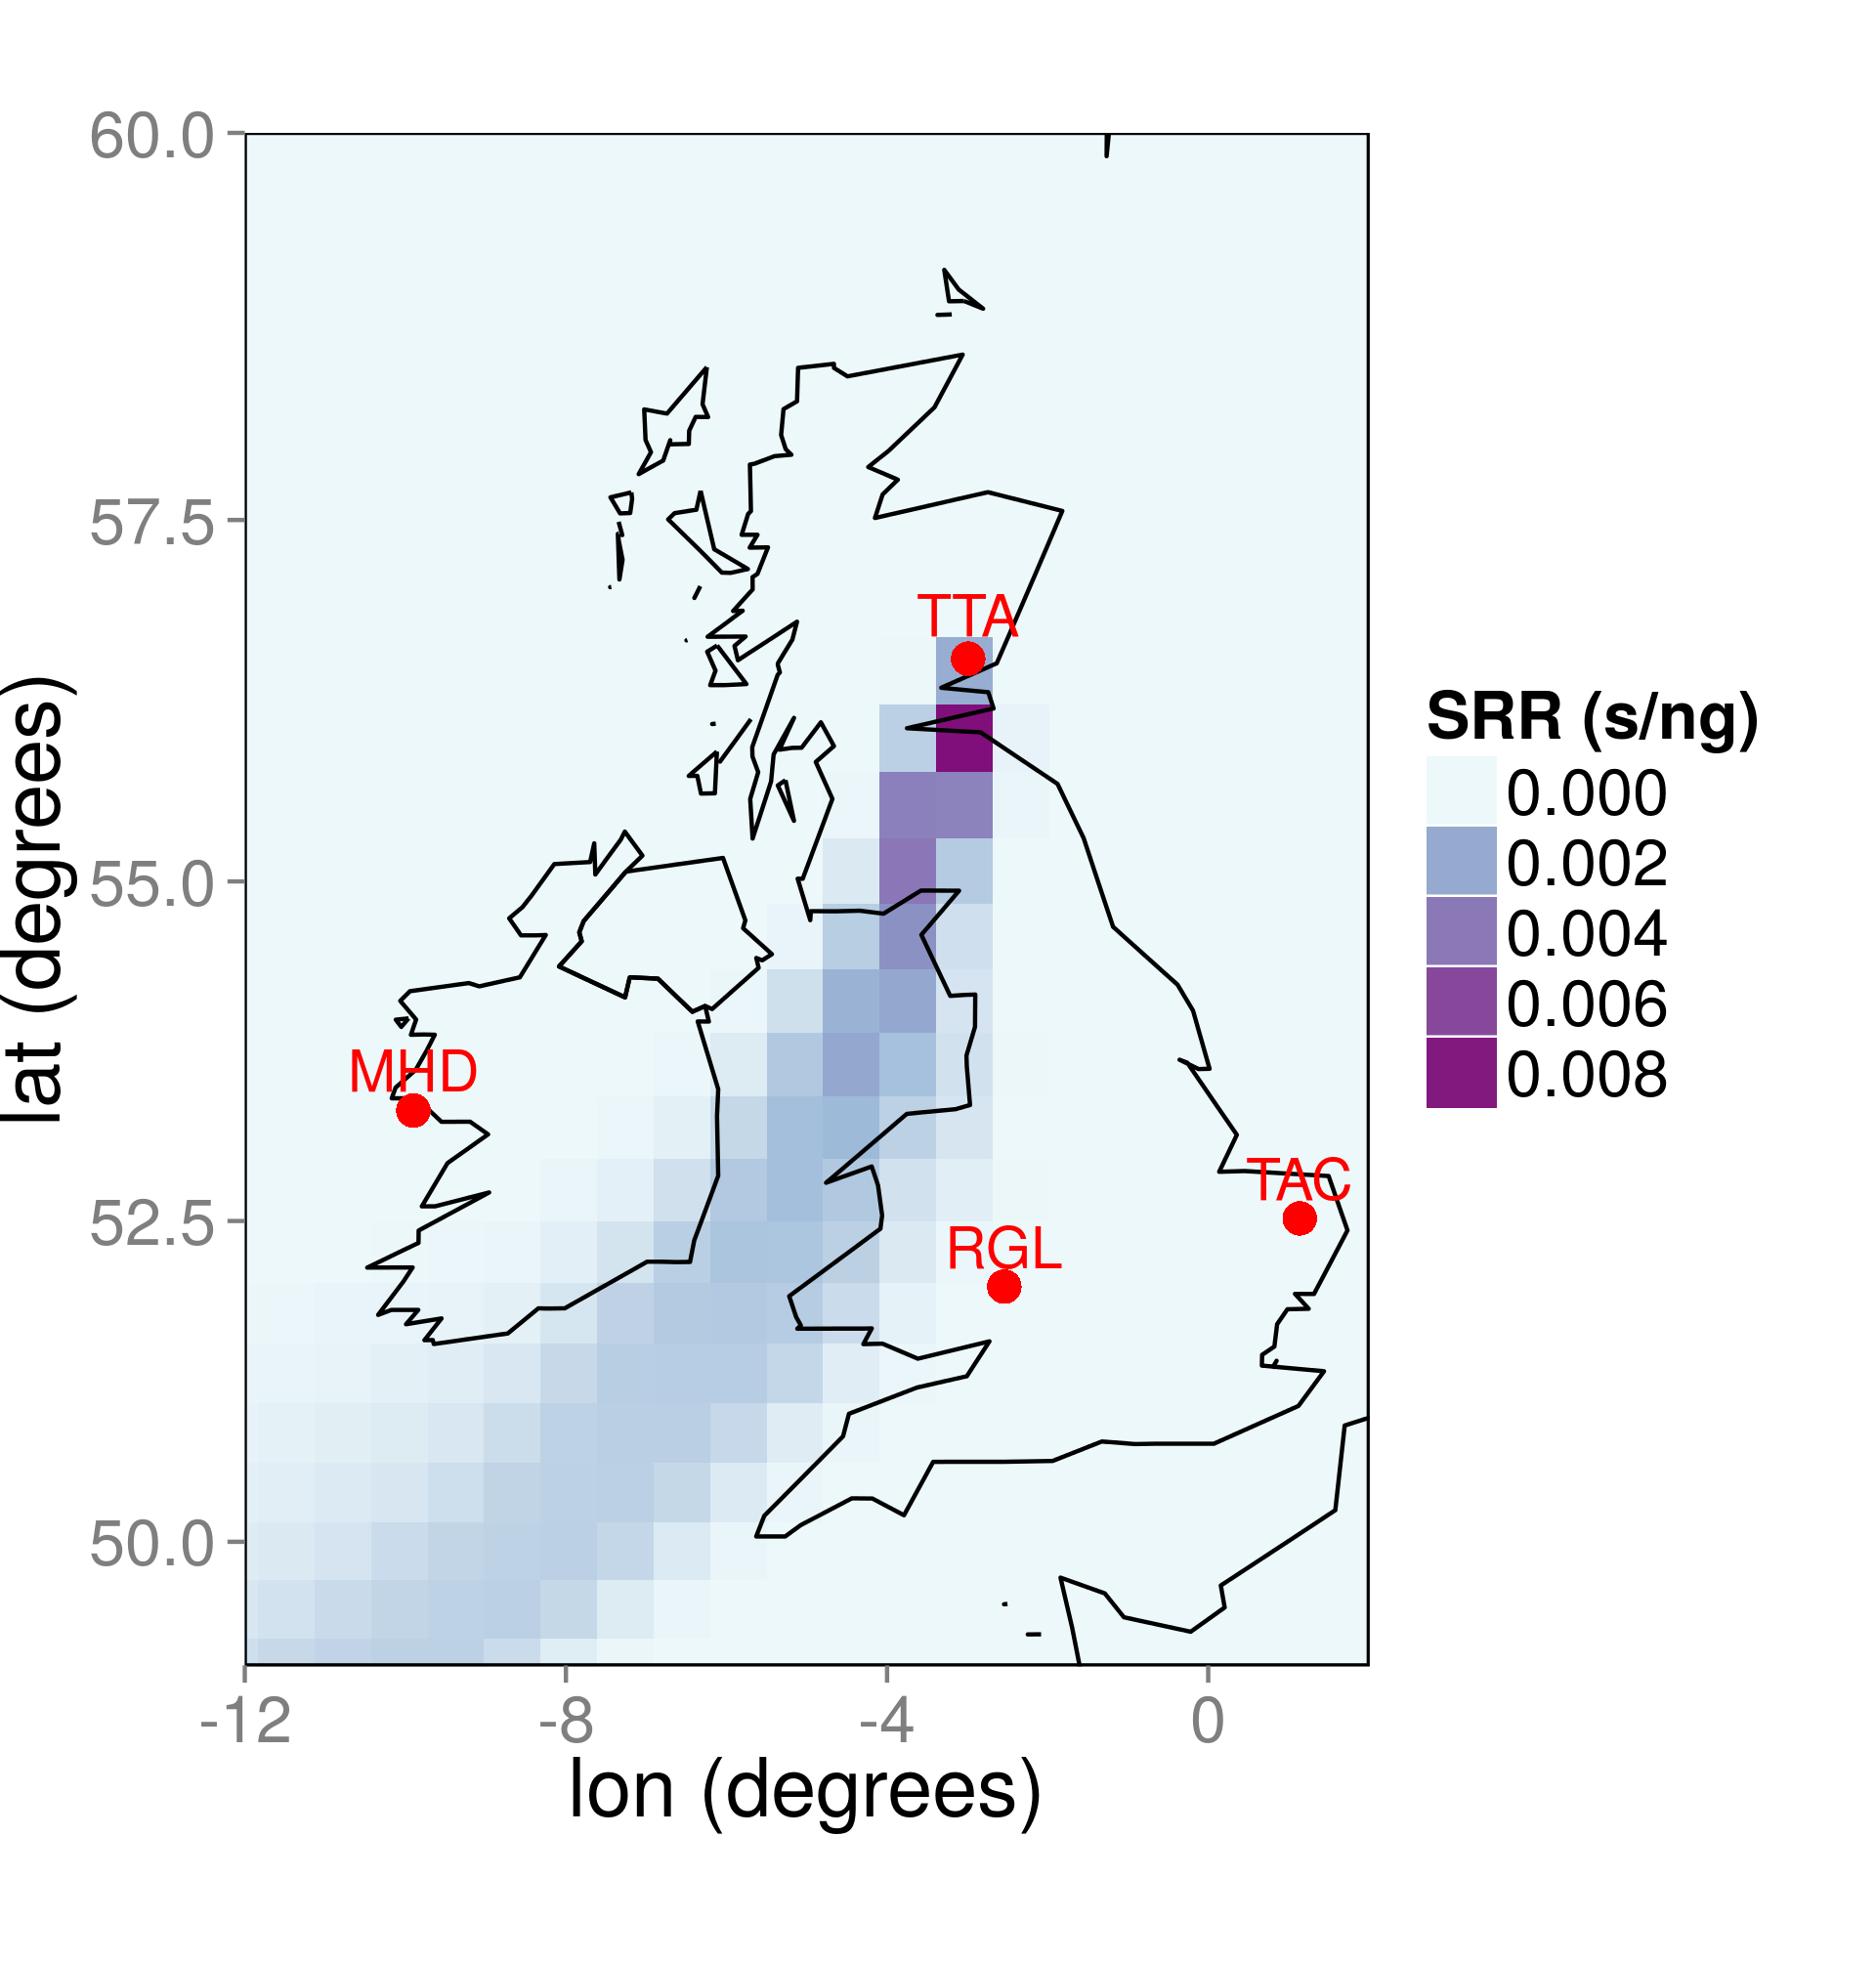
\includegraphics[width=1.4in]{TTA_01_01.png}


\end{column}
\end{columns}
\end{frame}


% #####################

% \begin{frame}
% \frametitle{Isolated measurements}

% \begin{center}
% \begin{figure}
% 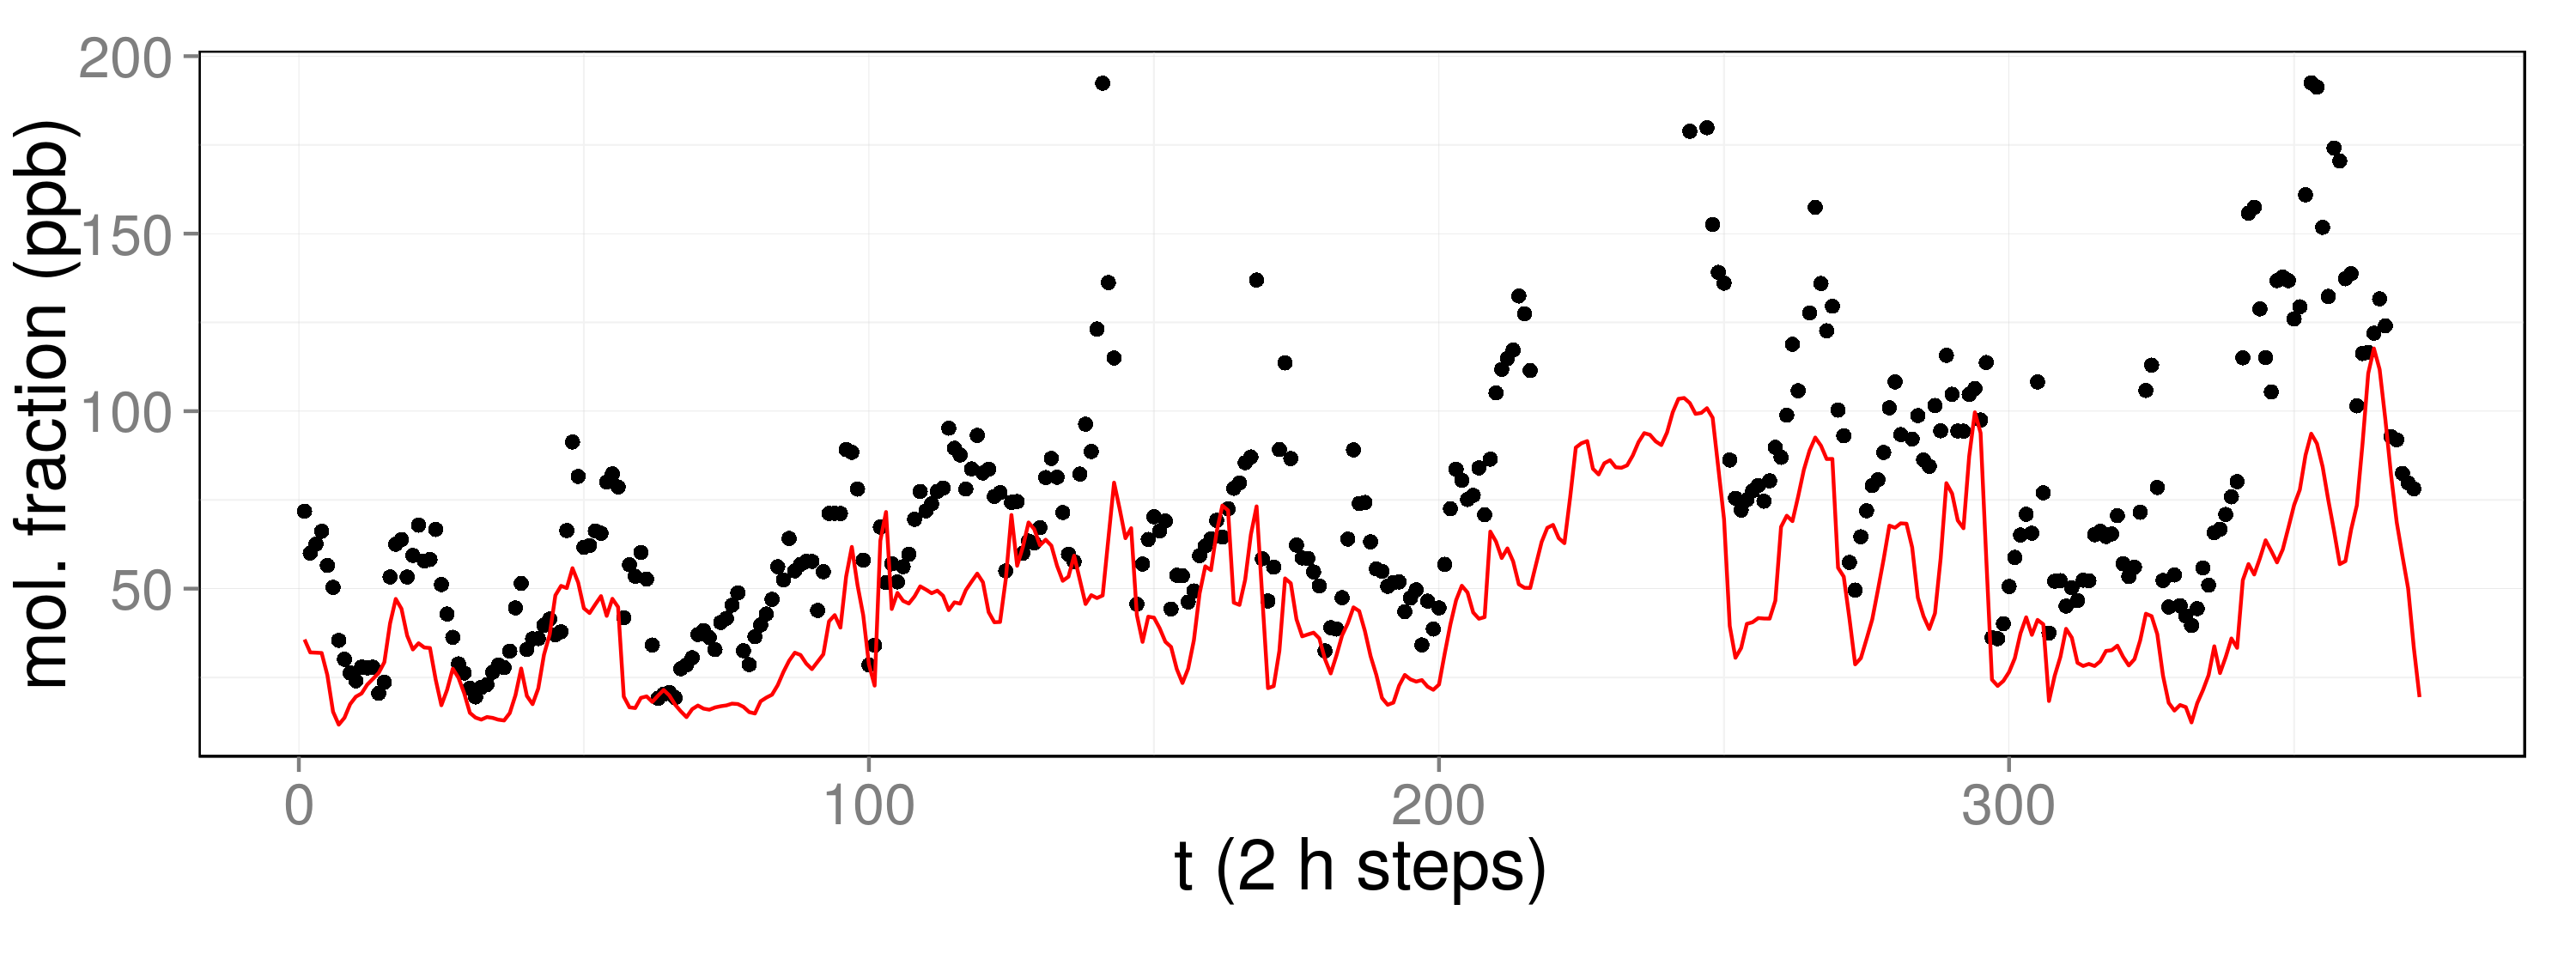
\includegraphics[width=3.5in]{TAC_01.png}
% \caption{Measurements of methane mole fraction in parts per billion (ppb) at Tacolneston, England (TAC) for January 2014, following background-removal (black dots) together with a forward-model prediction (red line) using NAME and the methane flux inventory. Each time step corresponds to an interval of 2 h.}
% \end{figure}
% \end{center}

% \vspace{-1cm}

% %\begin{itemize}
% %\small
% %\item The inversion is an ill-posed problem: We need to estimate a (spatial) emissions field from measurements that aggregate spatio-temporally.
% %\item Current methods use data assimilation methods with prior expectations set to what is reported in the inventories.
% %\item Inversions are sometimes orders of magnitude off.
% %\end{itemize}

% \normalsize

% \end{frame}

\begin{frame}
\frametitle{Challenges / current state-of-the-art}

\begin{itemize}
\item Not use the inventory as a prior (try a spatially invariant prior). \vfill
\item Not assume Gaussianity of the flux field.\vfill
\item Not assume independence of flux at the locations of interest.\vfill
\item Not assume that the LPDM is perfect.\vfill
\end{itemize}
\end{frame}

\subsection{Lognormal spatio-temporal model}

\begin{frame}
\frametitle{Hierarchical modelling framework}

\begin{itemize}
\item Observation model:
\begin{equation}\label{eq:obs}
Z_{m,t}(\svec) = Y_{m,t}(\svec) + \varepsilon_{m,t}(\svec); \quad \svec \in D^O_{m,t}; \quad t \in \mathcal{T}.
\end{equation}

\item Mole-fraction process model:
\begin{equation}\label{eq:mv}
Y_{m,t}(\svec) = \int_D b_t(\svec,\uvec)Y_f(\uvec)\intd\u + \zeta_{t}(\svec); \quad \svec \in D;\quad t \in \mathcal{T}.
\end{equation}

\item Flux process model:
\begin{equation}
Y_f(\svec) \sim \mathcal{LGP}(\widetilde\mu_f(\s;\varthetab),\widetilde{C}_{\ff}(\s,\u; \varthetab)); \quad \svec,\uvec \in D.
\end{equation}
\end{itemize}
\end{frame}


\begin{frame}
\frametitle{Bivariate lognormal spatial model for the flux field}

\begin{itemize}
\item Let $Y_f(\svec) \equiv \exp(\widetilde{Y_f}(\svec))$ be a lognormal spatial process.\vfill \pause
\item Then, if $\E(\widetilde{Y}_f(\s)) \equiv \widetilde\mu_f(\s;\varthetab)$ and $\cov(\widetilde{Y}_f(\s),\widetilde{Y}_f(\u)) \equiv \widetilde{C}_{\ff}(\s,\u; \varthetab)$.


\begin{align*}
\mu_f(\s;\varthetab) &\equiv \E(Y_f(\s)) \\ &=  \exp(\widetilde{\mu}_f(\svec;\varthetab) + (1/2)\widetilde{C}_{\ff}(\s,\s;\varthetab)); \quad \svec \in D,\\
&\\
 C_{\ff}(\s,\u;\varthetab) &\equiv \cov(Y_f(\s),Y_f(\u))
\\&= \mu_f(\s;\varthetab)\mu_f(\u;\varthetab)[\exp(\widetilde{C}_{\ff}(\s,\u;\varthetab)) - 1] ; \quad \svec,\uvec \in D.
\end{align*} \vfill
\end{itemize}

\end{frame}


\begin{frame}
\frametitle{Lognormal bivariate model}

\begin{itemize}

\item We have a spatio-temporal bivariate model:

\begin{align*}
\E\left(Y_{m,t}(\s)\mid Y_f(\cdot)\right)&\,=\int_D{b_t(\s,\v)Y_f(\v)\,\d \v};\quad \s\in D,\\
\cov\left(Y_{m,t}(\s),Y_{m,t'}(\u)\mid Y_f(\cdot)\right)&\,=C_{m\mid f,t,t'}(\s,\u);\quad \s,\u\in \mathbb{R}^d,
\end{align*}

\pause with the mole-fraction covariance:
\begin{equation*}
C_{mm,t,t'}(\s,\u) = C_{m\mid f,t,t'}(\s,\u)+\int_D\int_D {\red{b_t(\s,\v)}} \blue{C_{\ff}(\v,\w)} \red{b_{t'}(\w,\u)}\d\v\d\w.
\end{equation*}

%\item The conditional covariance $C_{m\mid f,t,t'}$ is used to account for simulator discrepancy (boundary conditions, model discretisation, linearisation, etc.).

\end{itemize}

\end{frame}


\begin{frame}
\frametitle{Expectations and covariances}

\vspace{-0.2in}

\begin{align*}
\Yvec_t(\cdot) \sim \Dist\begin{pmatrix} \begin{pmatrix} \mu_f(\cdot) \\ \mu_{m,t}(\cdot) \end{pmatrix},\begin{pmatrix}  C_{\ff}(\cdot,\cdot) &  C_{fm,t'}(\cdot,\cdot) \\  C_{mf,t}(\cdot,\cdot) &  C_{mm,t,t'}(\cdot,\cdot) \end{pmatrix} \end{pmatrix},\quad t,t' \in \mathbb{R}^+.
\end{align*}

\begin{itemize}
\item \small Is the cross-covariance function matrix (CCFM) nonnegative-definite? \pause
\item \small Consider two spatial processes $Y_1^0(\svec)$, $Y_2^0(\svec)$ and interaction function $b(\svec,\uvec)$. The CCFM is nonnegative-definite if, for any $n_1,n_2$ such that $n_1 + n_2 > 0$, any locations $\{\svec_{1k}\}, \{\svec_{2l}\}$ and any real numbers $\{a_{1k}\},\{a_{2l}\}$,

\footnotesize
\begin{equation*}
 \var\left(\sum_{k=1}^{n_1}{a_{1k}Y_1^0(\s_{1k})}+\sum_{l=1}^{n_2}{a_{2l}Y_2^0(\s_{2l})}\right)  \ge 0.
\end{equation*}


%\item Our problem is the size of $\bSigma$, which can become very large.
% \item What to choose for $C_{2|1,t,t'}(\svec,\uvec)$? \vfill
% \item \emph{Strategy 1}: If dim$(\Zvec_{2,t}) < 10$, say, then use standard spatio-temporal covariance functions, which yield (dense) covariance matrices, and evaluate $Y_{2,t}(\cdot)$ only where we take observations. \vfill
% \item \emph{Strategy 2}: If dim$(\Zvec_{2,t}) \gg 10$, then we need to use sequential estimation methods,  dimensionality reduction and/or {\bf matrix sparsity}. \vfill
\end{itemize}
\end{frame}


\begin{frame}
\frametitle{Is the bivariate model always valid?}

\small
\begin{itemize}
\item It can be shown that
\begin{align*}
& \var\left(\sum_{k=1}^{n_1}{a_{1k}Y_1^0(\s_{1k})}+\sum_{l=1}^{n_2}{a_{2l}Y_2^0(\s_{2l})}\right)\\
&= \sum_{l=1}^{n_2}\sum_{l'=1}^{n_2}a_{2l}a_{2l'}C_{2\mid 1}(\s_{2l},\s_{2l'})+\int_D \int_D{\red{a(\s)a(\u)}\blue{C_{11}(\s,\u)}\,\d\s\d\u},
\end{align*}
where
\begin{equation*}
a(\s)\equiv \sum_{k=1}^{n_1}a_{1k}\delta(\s-\s_{1k})+\sum_{l=1}^{n_2}a_{2l}b(\s_{2l},\s);\quad \s\in \RR^d.
\end{equation*}
\item For details and proof for $p$-variate processes see Cressie and Zammit-Mangion (\url{http://arxiv.org/abs/1504.01865}).

\end{itemize}
\end{frame}


\begin{frame}
\frametitle{Model 1}

\begin{itemize}

\item The discrepancy is a separable spatio-temporal Gaussian process with
\begin{align*}
C_{m|f,t,t'}(\svec,\uvec) &= \sigma^2_{m|f}\rho_s(\svec,\uvec; d)\rho_t(t,t'; a),\\
\rho_s(\svec,\uvec; d) &\equiv \exp(\| \svec - \uvec \| / d);\quad d>0, \\
\rho_t(t,t'; a) &\equiv a^{|t - t'|}; \quad |a| < 1.
\end{align*}

\item Then $\bSigma_{m|f} = \sigma^2_{m|f} \widetilde\bSigma_{m|f,t} \otimes \widetilde\bSigma_{m|f,s}$.
\item $\Bmat$ is obtained by concatenating $\{\Bmat_t: t = 1,2,\dots\}$
\begin{equation*}
\bSigma =
\begin{pmatrix}
\bSigma_{\ff} & \bSigma_{\ff}\Bmat' \\
\Bmat \bSigma_{\ff} & \Bmat \bSigma_{\ff}\Bmat' + \bSigma_{m|f}
\end{pmatrix}.
\end{equation*}.

% \item $\Bmat$ is dense: Sparse covariance matrices are not computationally helpful.

\end{itemize}

\end{frame}


% \begin{frame}
% \frametitle{Model 2}

% \begin{equation*}
% \bSigma^{-1} = \begin{pmatrix}
% \Bmat'\Qmat_{2|1}\Bmat + \Qmat_{11} & -\Bmat'\Qmat_{2|1} \\
% -\Qmat_{2|1}\Bmat & \Qmat_{2|1}
% \end{pmatrix}.
% \end{equation*}

% \begin{itemize}
% \item Large benefit by making sure the (very large) matrix $\Qmat_{2|1}$ is sparse.
% \pause \item We define
% \begin{equation*}
% \Qmat_{2|1} \equiv \sigma_{2|1}^{-2}\widetilde\Qmat_{2|1,t} \otimes \widetilde\Qmat_{2|1,s}~~,
% \end{equation*}
% \noindent where
% \begin{equation*}
% \widetilde\Qmat_{2|1,t} \equiv \begin{pmatrix} 1 & -a &0&&&& 0\\ -a & (1 + a^2) & -a &&&&0  \\ &&&\ddots&&& \\ 0&&&& -a& (1 + a^2) & -a \\ 0&&&&0&-a & 1 \end{pmatrix}.
% \end{equation*}
% \noindent and we get $\Qmat_{2|1,s}$ from an intrinsic Gaussian Markov random field specification.
% \end{itemize}
% \end{frame}

% \begin{frame}
% \frametitle{$\bSigma^{-1}$ is sparse}

% \vspace{-0.1in}

% \begin{equation*}
% \bSigma^{-1} = \begin{pmatrix}
% \Bmat'\Qmat_{2|1}\Bmat + \Qmat_{11} & -\Bmat'\Qmat_{2|1} \\
% -\Qmat_{2|1}\Bmat & \Qmat_{2|1}
% \end{pmatrix}.
% \end{equation*}

% \begin{figure}
% 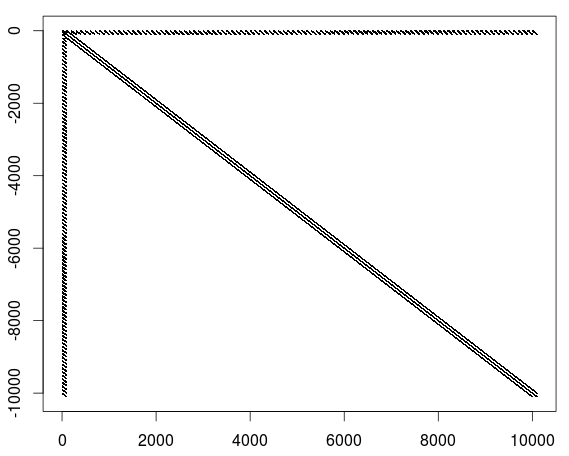
\includegraphics[width=1.8in]{Qsparse.png}
% \caption{Sparsity pattern of $\bSigma^{-1}$. Note how the top-left, top-right and bottom-left blocks are dense. The largest block, $\Qmat_{2|1}$ is very sparse due to its (sparse) Kronecker structure.}
% \end{figure}
% \end{frame}

\subsection{Inference}

\begin{frame}
\frametitle{Inference}

\begin{itemize}
\item Interaction function (transport model) $b_t(\svec,\uvec)$ is assumed known from NAME. \vfill
\item We can obtain reasonable estimates of the parameters appearing in $C_{\ff}(\svec,\uvec)$ from inventories (range, marginal variance, and nugget). \vfill
\item We have no idea what the parameters appearing in $C_{m|f}(\svec,\uvec)$ are. We estimate these using an approximate EM algorithm. Flux prediction is done using Hamiltonian Monte Carlo (HMC).  \vfill
\end{itemize}
\end{frame}

% \begin{frame}
% \frametitle{Computational strategy}

% \begin{itemize}
% \item This is an ill-posed problem: In these sort of problems it is hard to obtain MCMC chains that mix well when both the parameters and the fields are unknown. \pause \vfill
% \item We know the first two moments -- use a {\bf Laplace-approximated-EM} to estimate the parameters, then fix the parameters and use MCMC for prediction. \vfill \pause
% \item This is known as an empirical hierarchical model \citep[EHM;][]{CressieWikle2011}. \vfill \pause
% \item We can compute all the (horrible) gradients analytically, so we use an MCMC method that takes advantage of these. This is known as Hamiltonian Monte Carlo (HMC). \vfill
% \end{itemize}
% \end{frame}

% \begin{frame}
% \frametitle{HMC}

% \begin{itemize}
% \item Use Hamiltonian dynamics to propose the next state in an MCMC chain \citep{Duane_1987}.
% \item Need knowledge of gradient to simulate dynamics.
% \item Suitable when variables are highly correlated \textit{a posteriori} (ill-posed problem).
% \item Dynamics are simulated using standard methods (Euler or leapfrog method).
% \item One-step updates = Langevin method.
% \item HMC chains are ergodic and reversible \citep{Neal_2011}.
% \item Available from \url{http://github.com/andrewzm/hmc}.
% \end{itemize}
% \end{frame}

% \begin{frame}
% \frametitle{HMC}

% \begin{center}
% 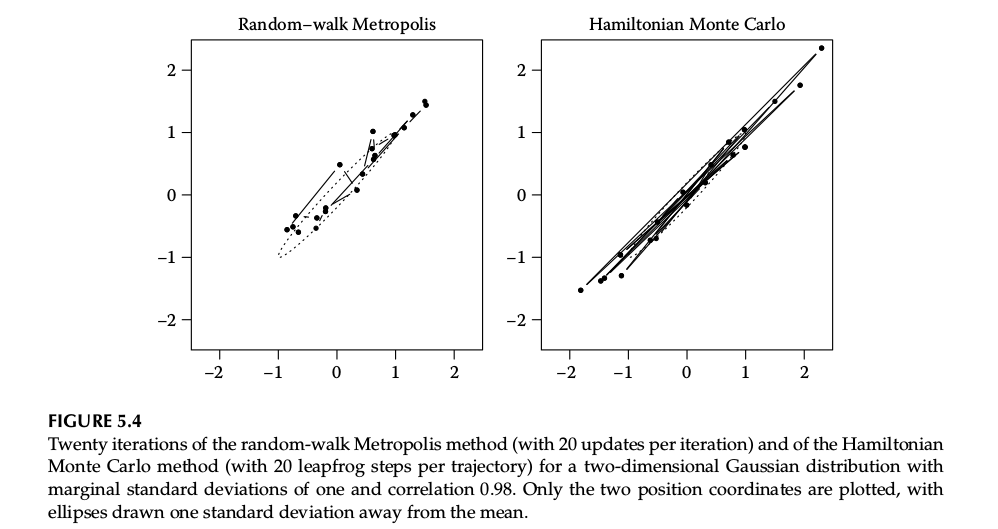
\includegraphics[width=4in]{HMC2.png}
% \end{center}
% \begin{itemize}
% \item Figure and caption taken from \cite{Neal_2011}.
% \end{itemize}
% \end{frame}


% \subsection{Simulation studies}


% \begin{frame}
% \frametitle{Simulation study}

% \begin{enumerate}
% \item Assume the properties of the lognormal flux spatial process (i.e., $\widetilde{C}_{11}$ and $\widetilde{\mu}_{1}$ are known), and simulate a realisation. \vfill
% \item Simulate a spatio-temporal interaction function (assumed known).\vfill
% \item Simulate mole fraction observations at a few locations (Model 1) and at many (1000) locations (Model 2).\vfill
% \item Infer the flux $Y_1(\svec)$ from the data in both cases.\vfill
% \end{enumerate}
% \end{frame}

% \begin{frame}
% \frametitle{Simulation study}

% \begin{itemize}
% \item Simulated interaction function.
% \end{itemize}

% \begin{figure}
% 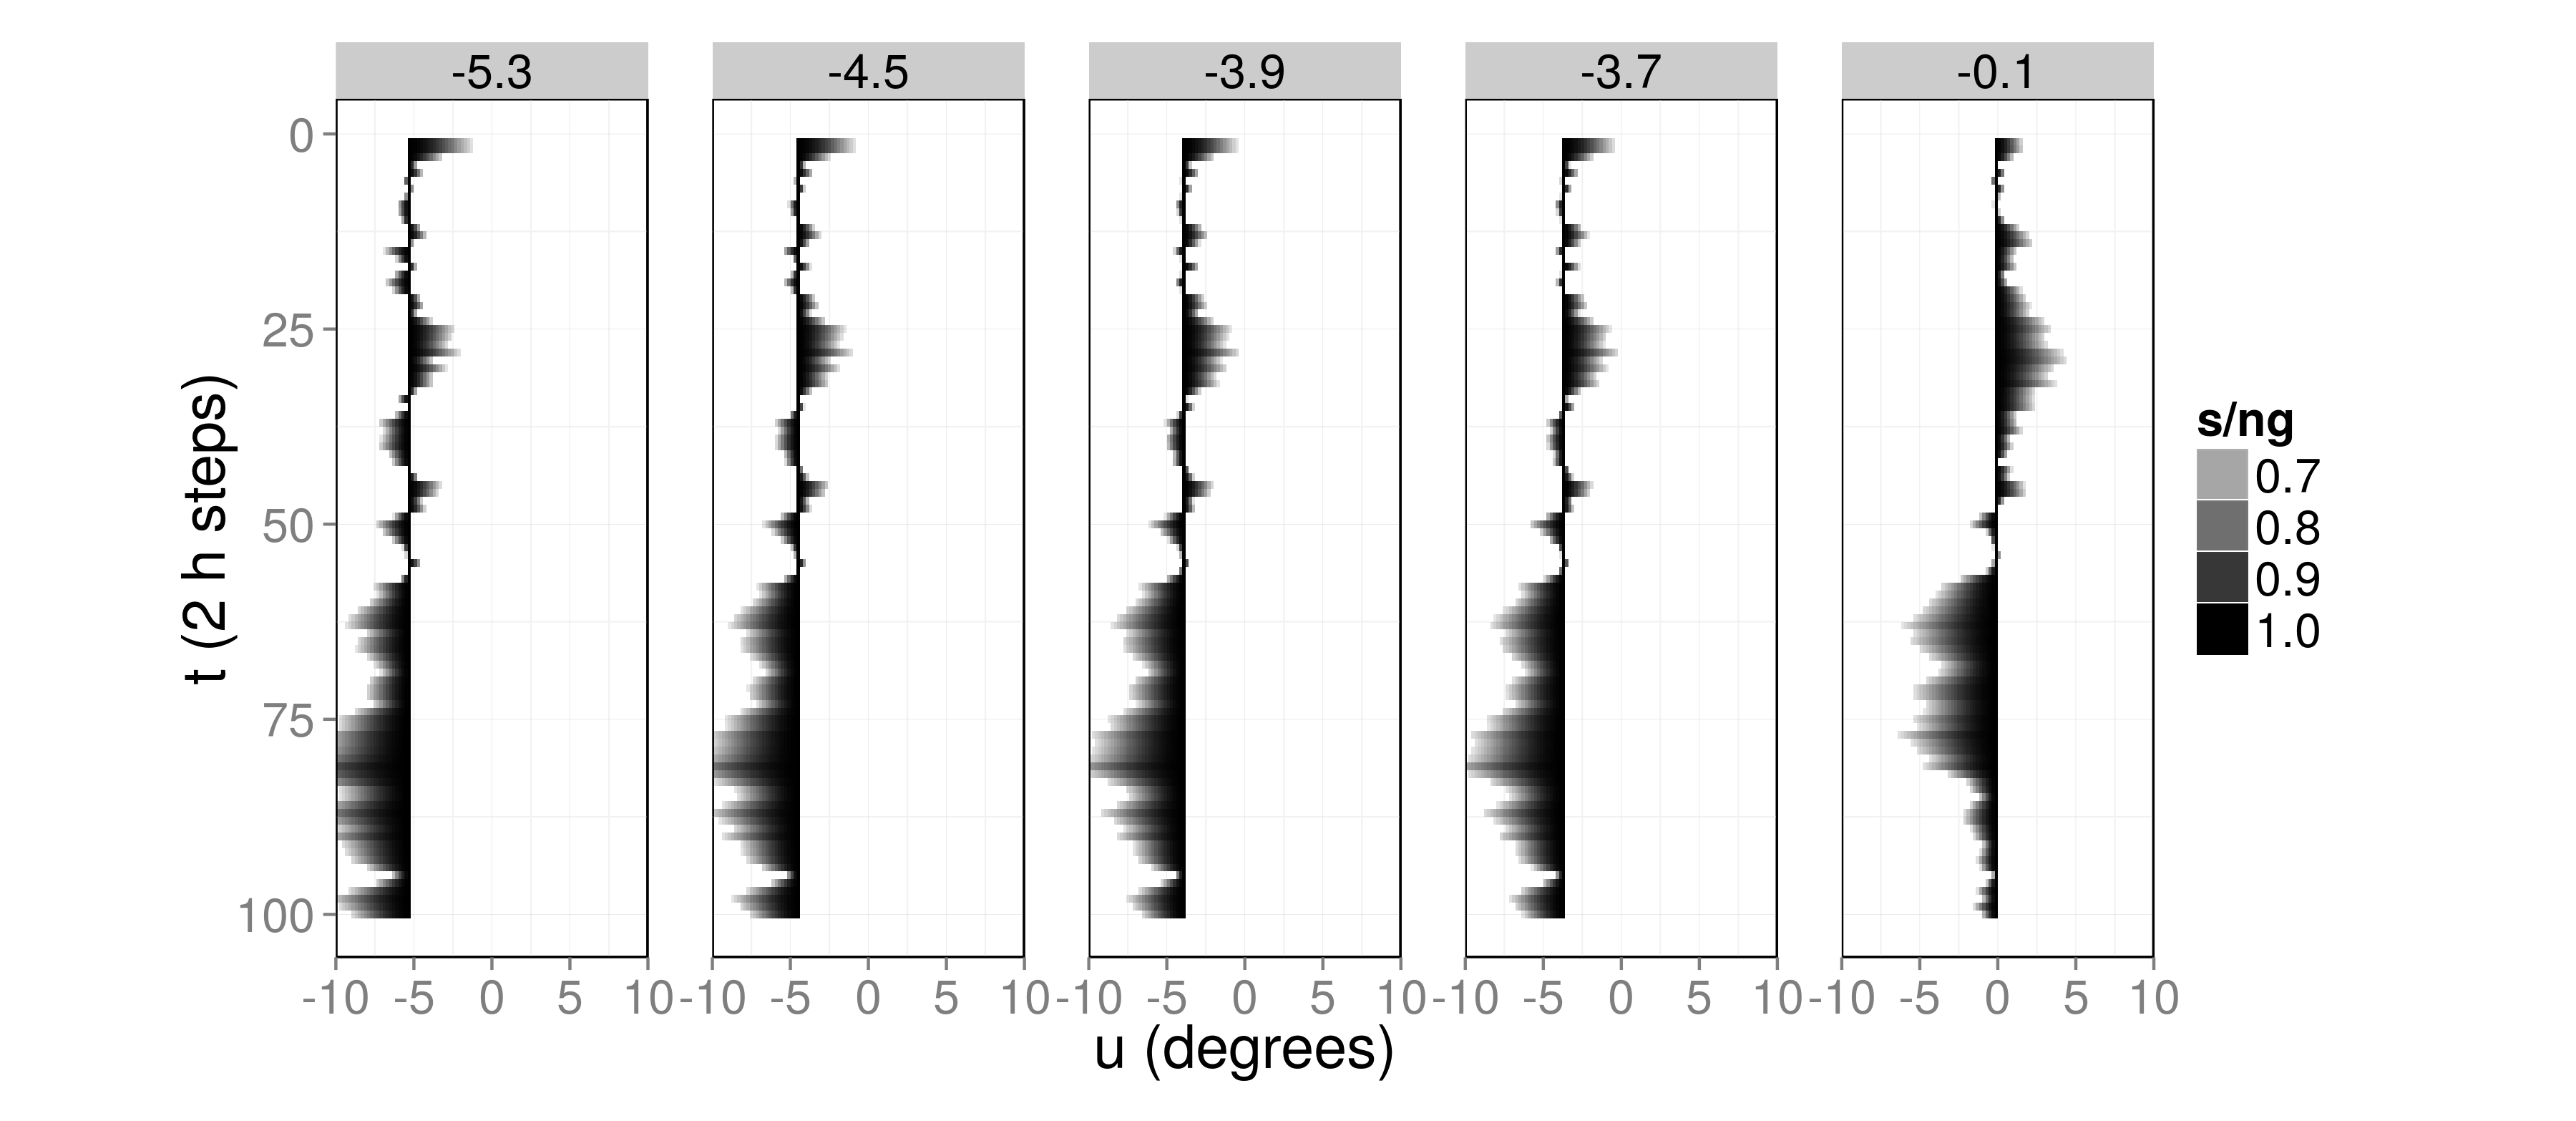
\includegraphics[width=4in]{B_plot.png}
% \caption{The source-receptor relationship $b_t(s,u)$ synthesised at five observation locations $s \in D^O_m = \{-5.3^\circ, -4.5^\circ,-3.9^\circ,-3.7^\circ,-0.1^\circ\}$.}
% \end{figure}
% \end{frame}

% \begin{frame}
% \frametitle{Simulation study}

% \begin{itemize}
% \item Flux and time-averaged mole-fraction field.
% \end{itemize}

% \begin{figure}
% 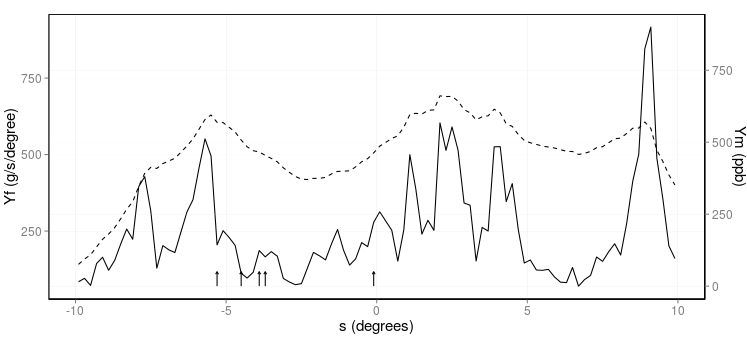
\includegraphics[width=4in]{Sim_plot2.png}
% \caption{A sample realisation of the flux field (solid line), the resulting mole-fraction field averaged over the entire temporal domain (dashed line) and the five observation locations (arrows).}
% \end{figure}
% \end{frame}


% \begin{frame}
% \frametitle{Simulation study}

% \begin{itemize}
% \item Laplace-EM proved relatively straightforward to implement.
% \item Convergence with Model 1 $\simeq$ 80 iterations.
% \item Convergence with Model 2 $\simeq$ 5 iterations (much more data).
% \item Convergence may be hard to achieve when mode is close to zero and tails are heavy.
% \item ``Bouncing method'' needs to be implemented for the HMC chain to respect positivity constraint on flux \citep{Neal_2011}.
% \end{itemize}
% \end{frame}


% \begin{frame}
% \frametitle{Simulation study}

% \begin{figure}
% 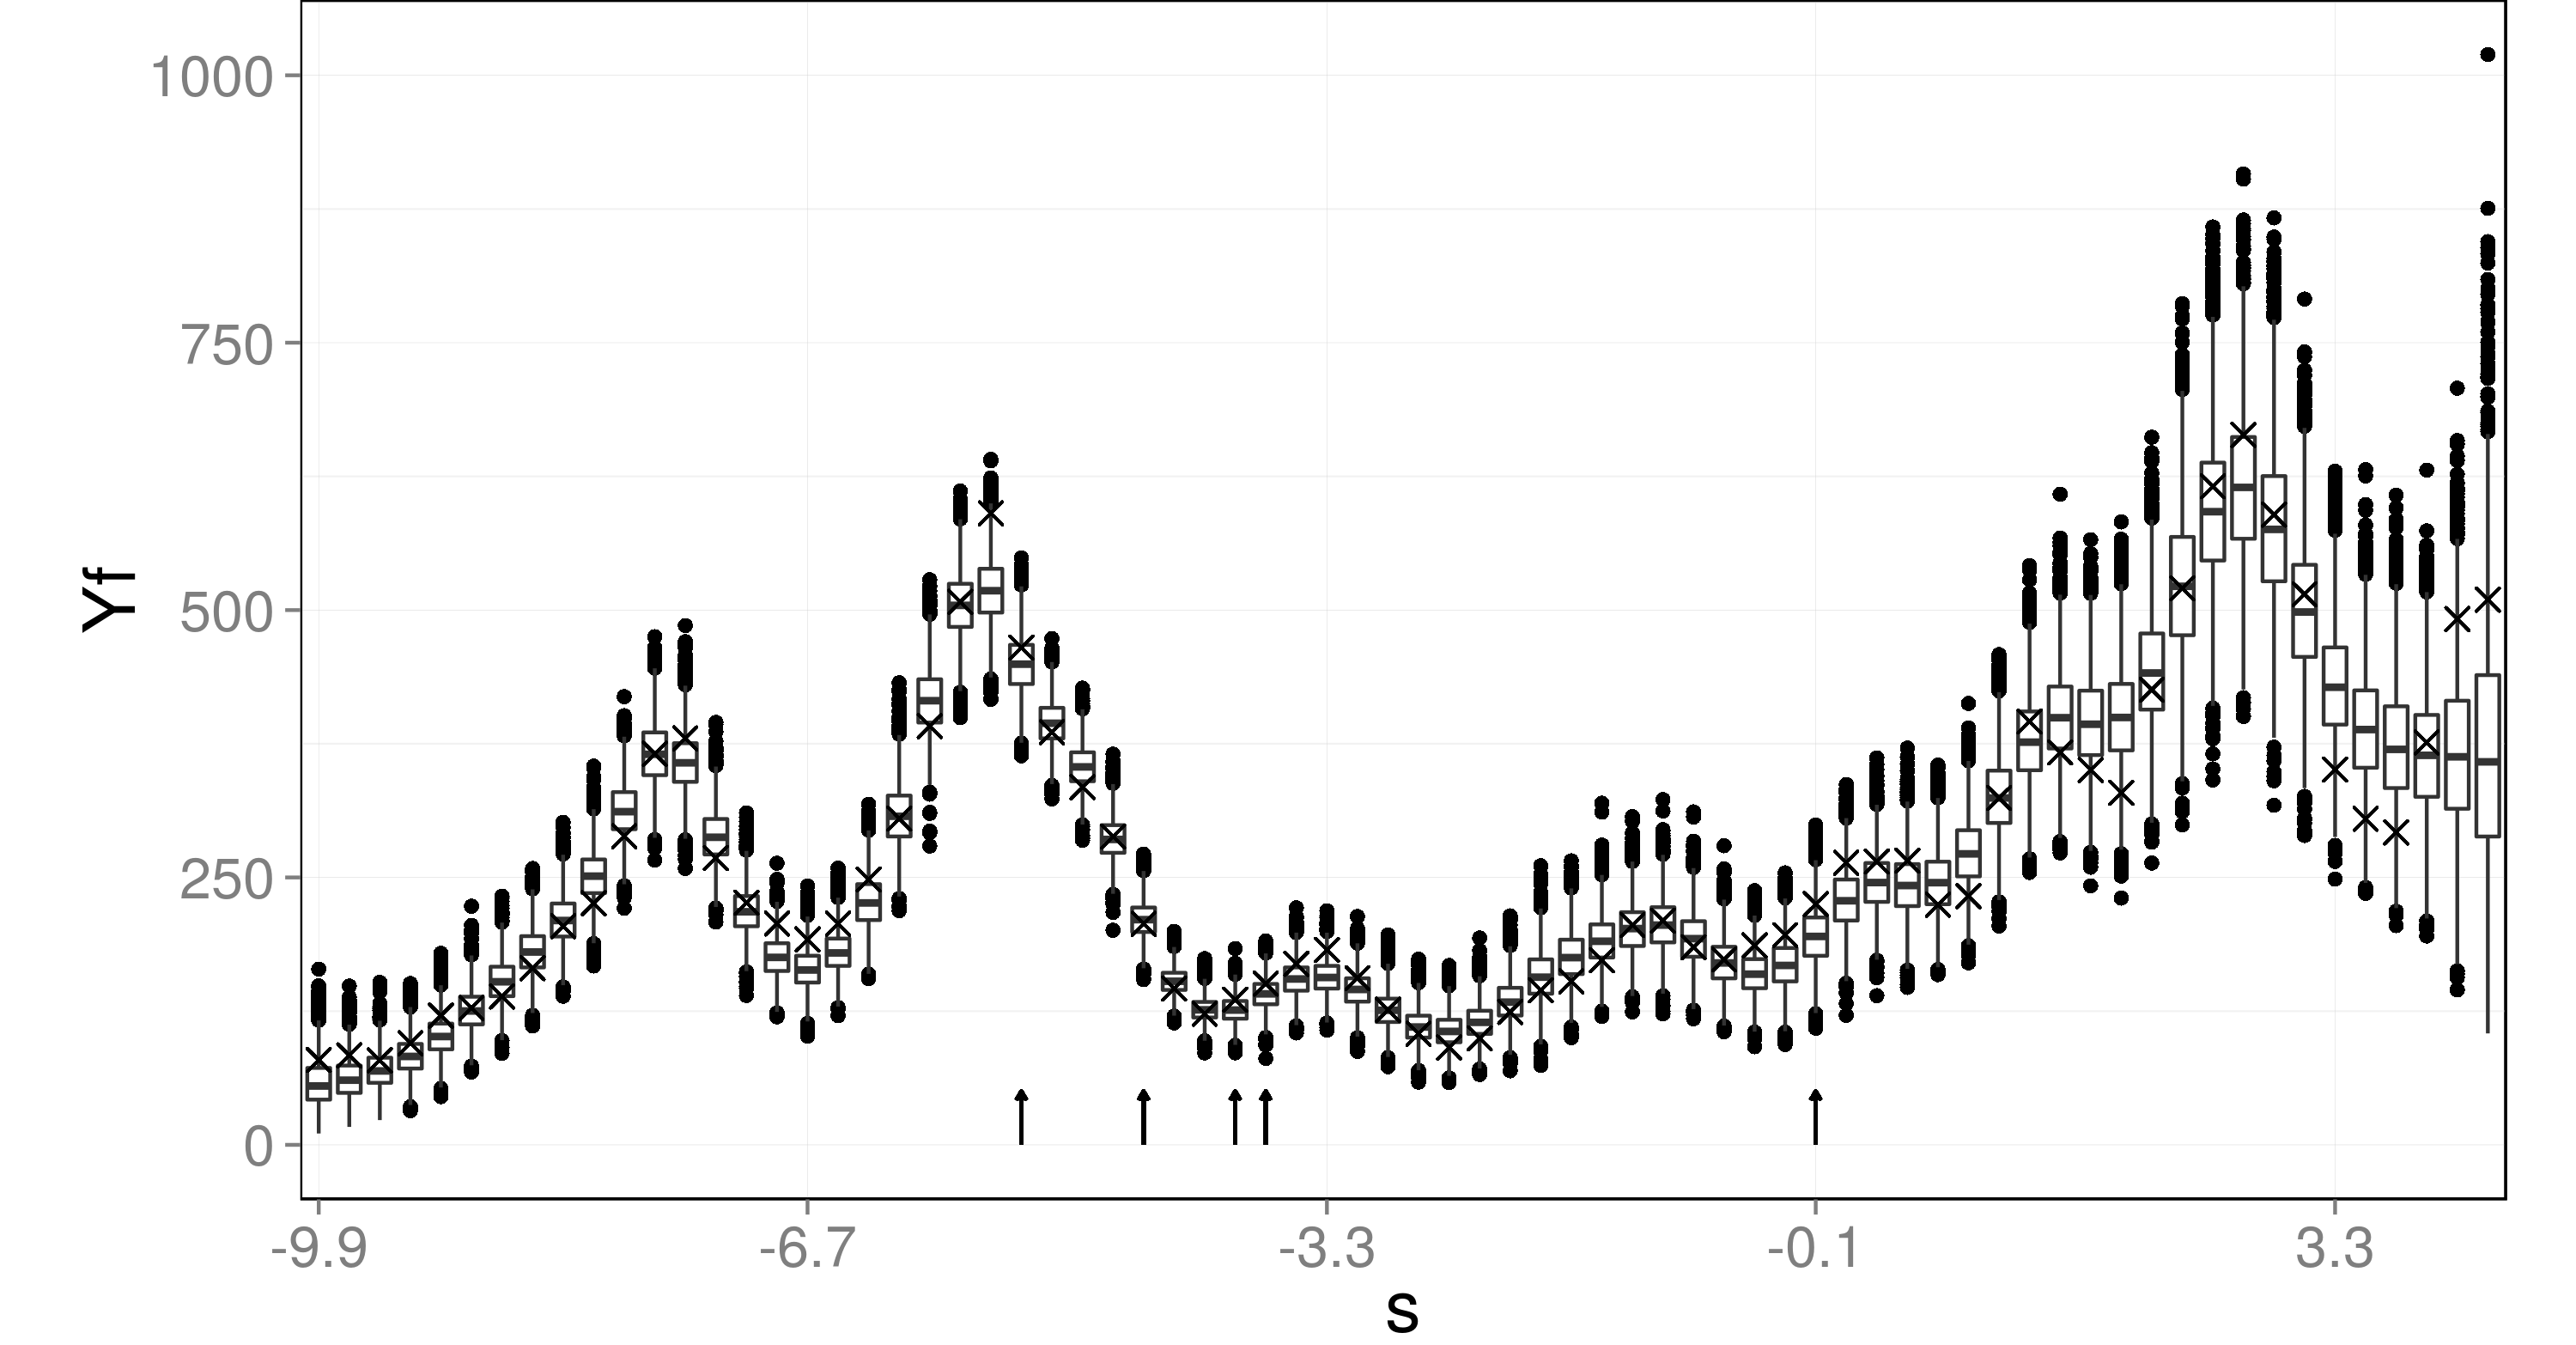
\includegraphics[width=3.7in]{Sim1_samples.png}
% \caption{Samples from the posterior distribution of the lognormal flux field obtained using Hamiltonian Monte Carlo (HMC). The crosses denote the true (simulated) fluxes, and the arrows denote the locations of the measurements. The vertical dashed lines show the spatial locations displayed in the next slide.}
% \end{figure}
% \end{frame}

% \begin{frame}
% \frametitle{Simulation study}
% \begin{itemize}
% \item Why include the HMC if we have a Laplace-EM algorithm?
% \end{itemize}
% \begin{center}
% \vspace{-0.5cm}
% \begin{figure}
% 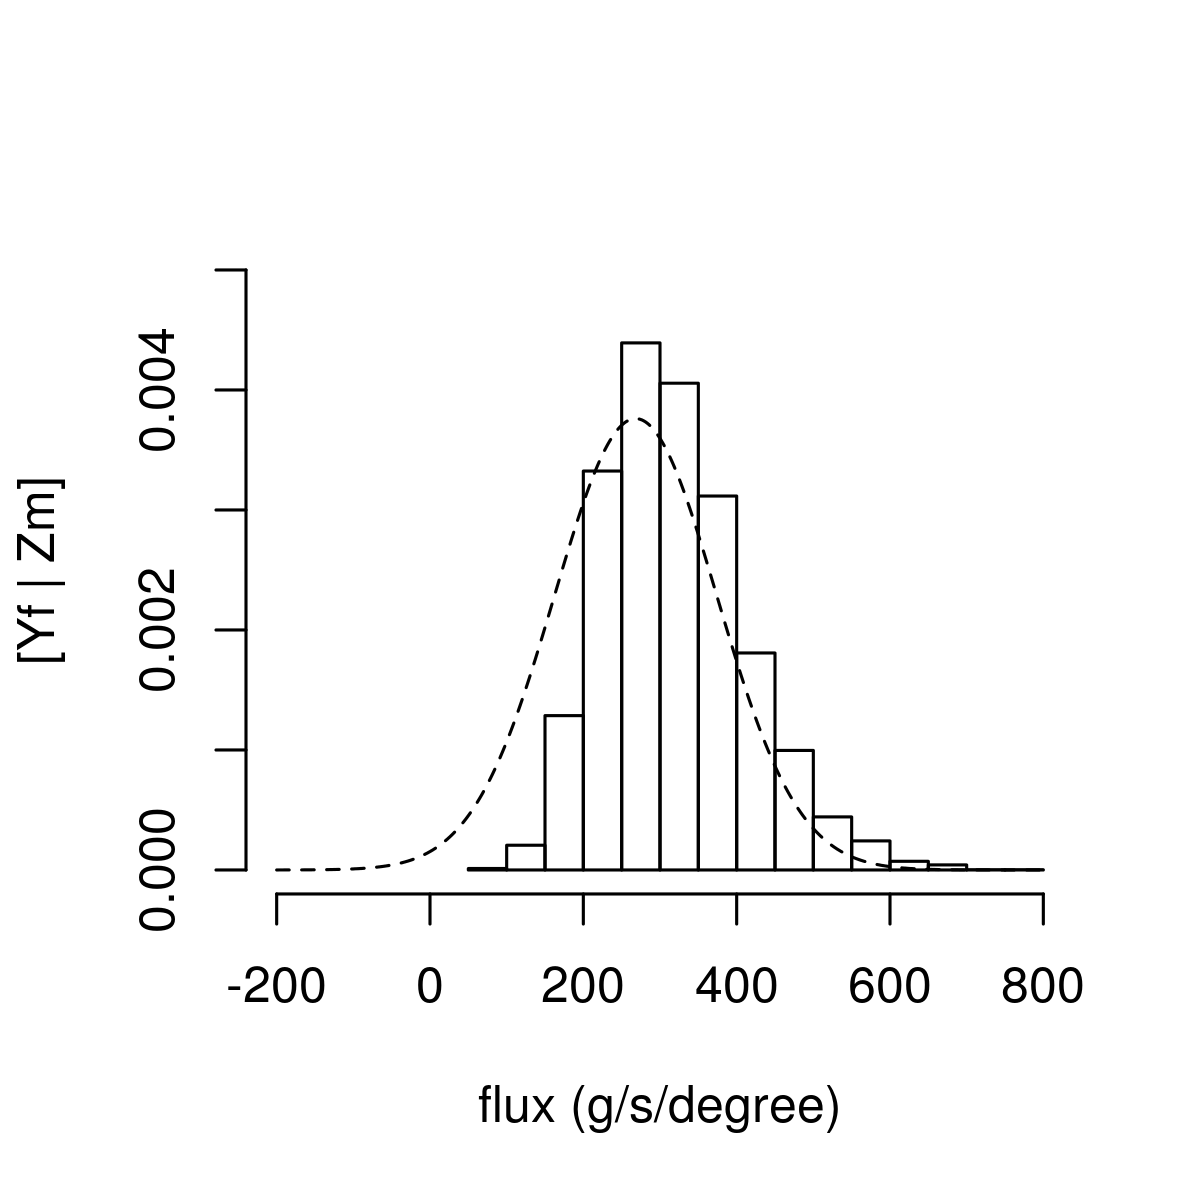
\includegraphics[width=2in]{density_sim1.png}
% 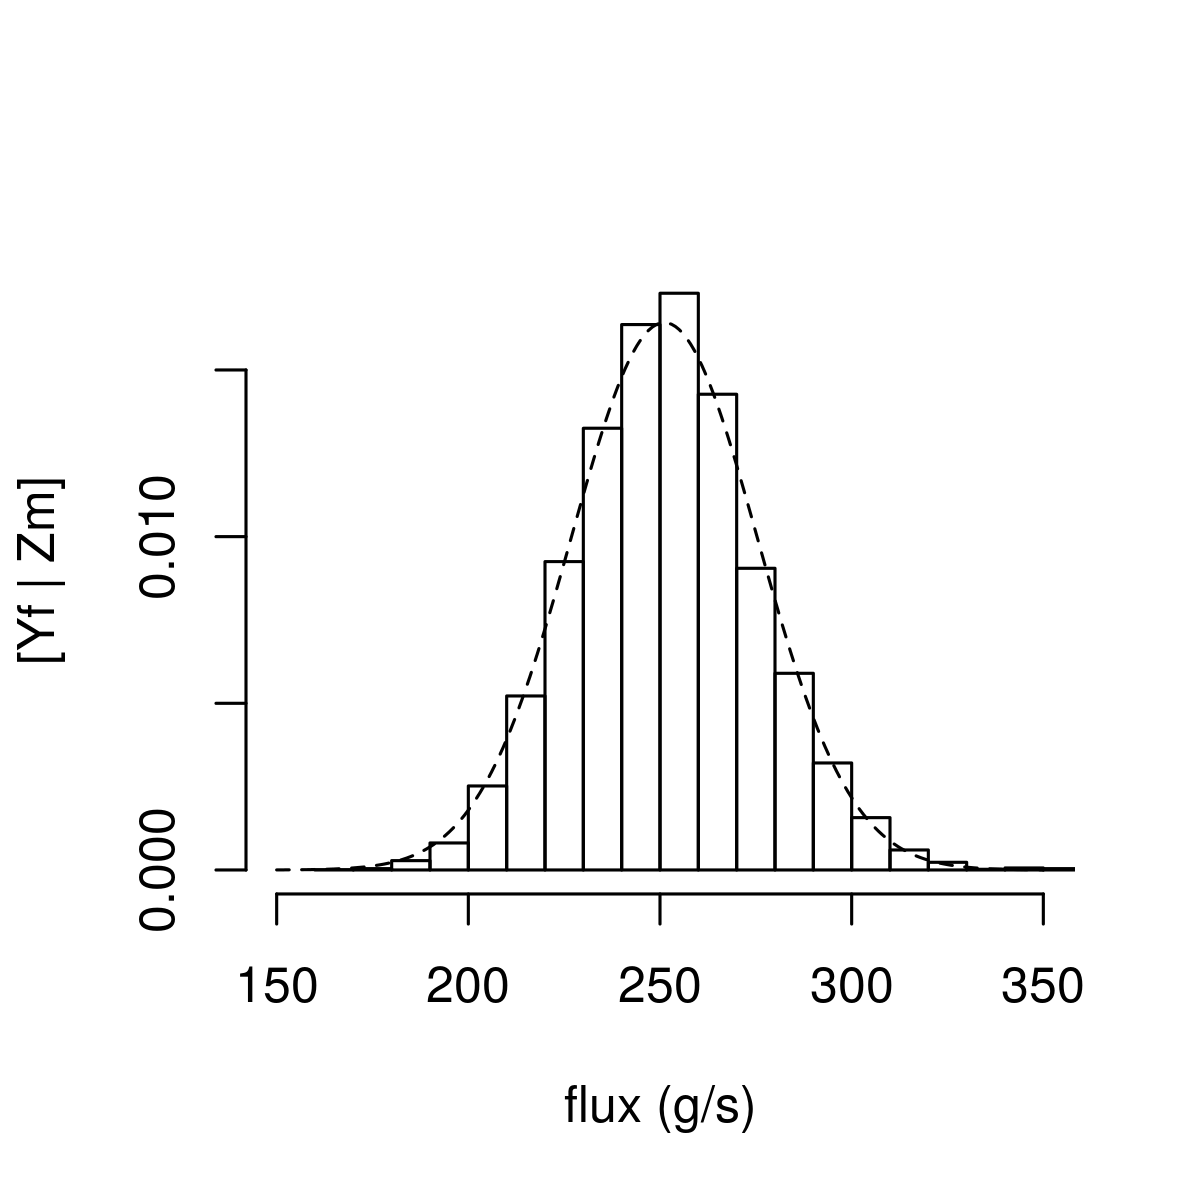
\includegraphics[width=2in]{density_sim10.png}
% 	\caption{Laplace approximation (dashed line) and a histogram of the empirical posterior distribution from the MCMC samples for the flux at $s = 3.9^\circ$ (left panel) and $s = -5.3^\circ$ (right panel).}
% \end{figure}
% \end{center}
% \end{frame}

\subsection{Case study: Methane emissions in the UK and Ireland}


% \begin{frame}
% \frametitle{UK and Ireland emissions}
% \begin{itemize}
% \item Extract spatial properties from the emissions inventory.
% \end{itemize}
% \begin{center}
% \vspace{-0.5cm}

% \begin{figure}
% 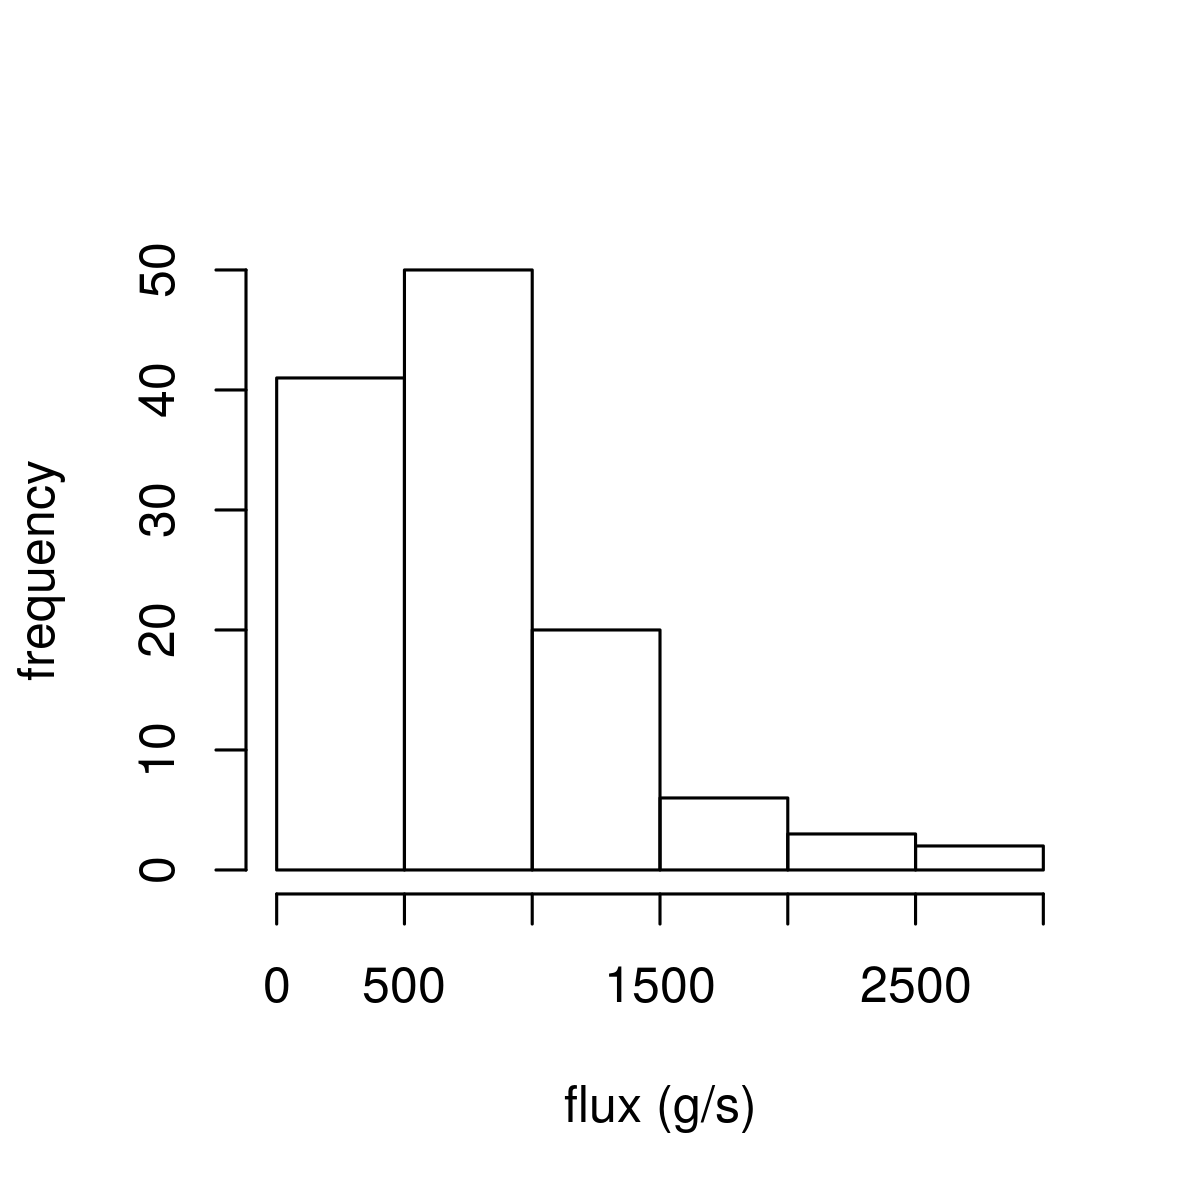
\includegraphics[width=2.0in]{histUK.png}
% 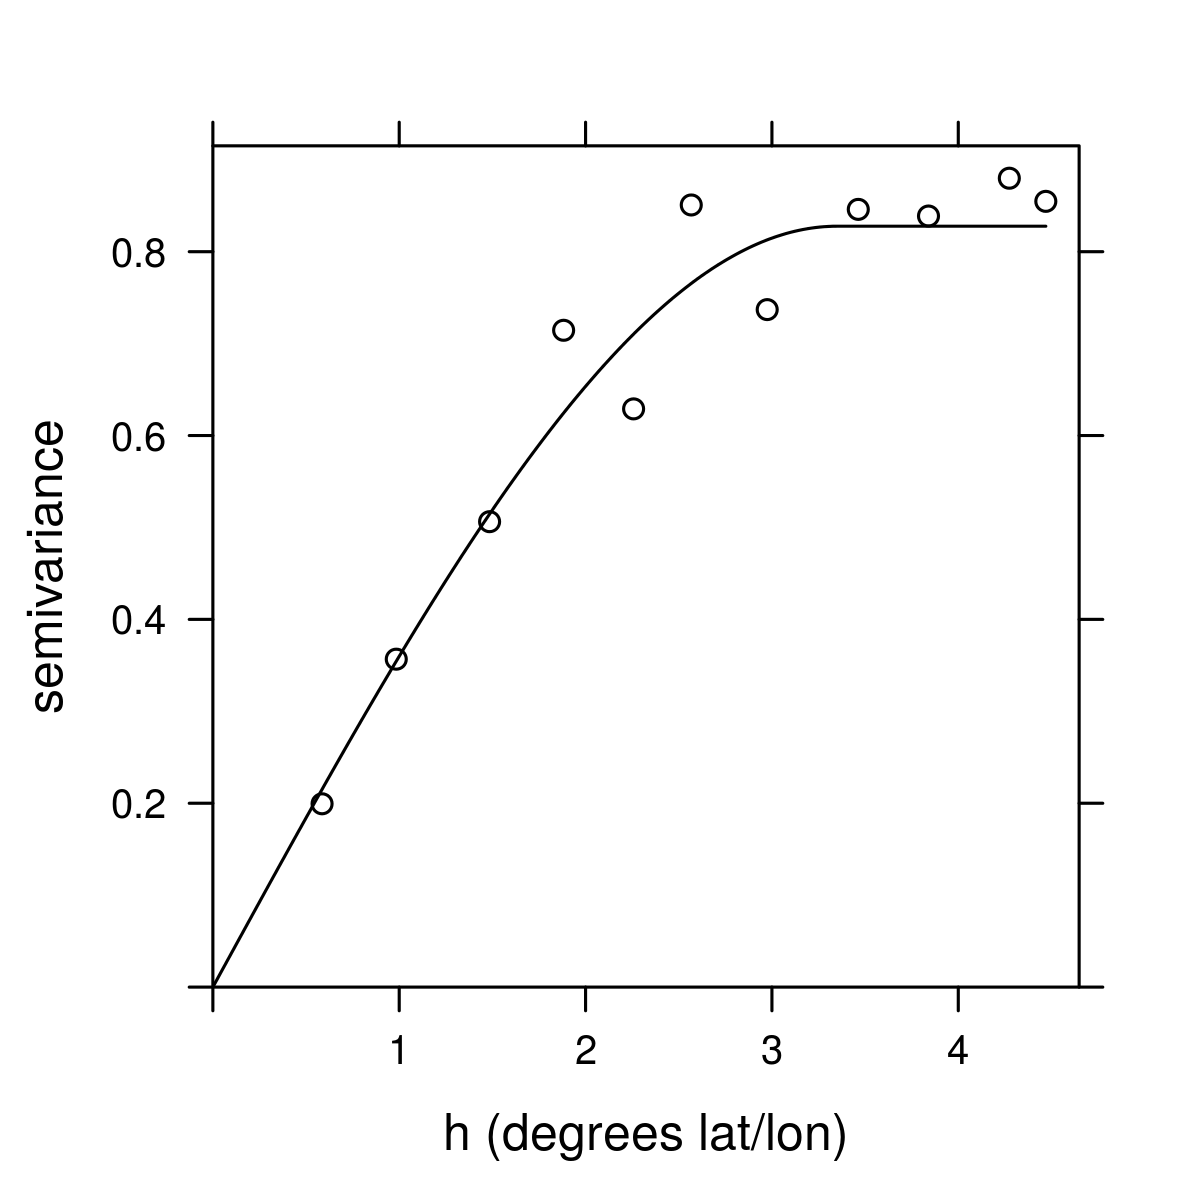
\includegraphics[width=2.0in]{variogram_est.png}
% 	\caption{Histogram of inventory fluxes in the UK and Ireland following regridding (left panel) and the empirical (open circles) and fitted (solid line) semi-variogram as a function of lag distance in degrees lat/lon. } \label{fig:var_est}
% \end{figure}
% \end{center}
% \end{frame}



\begin{frame}
\frametitle{UK and Ireland emissions}
\begin{itemize}
\item We set the prior-flux expectation to be spatially constant. \vfill
\item Laplace-EM converged in $\simeq$ 30 iterations. \vfill
\item Simulator discrepancy is not negligible: \vfill
\begin{enumerate}
\item $\hat\sigma_{2|1} \simeq 26$ ppb, (observation error $\simeq$  10 ppb)\vfill
\item $\hat d \simeq 200$ km, \vfill
\item $\hat a \simeq 0.97$ ($1/e$ rate of 66 h). \vfill
\end{enumerate}
\end{itemize}
\end{frame}

\begin{frame}
\frametitle{Posterior distribution of mole fractions}
\begin{center}
\vspace{-0.5cm}

\vspace{-0.1in}

\begin{figure}
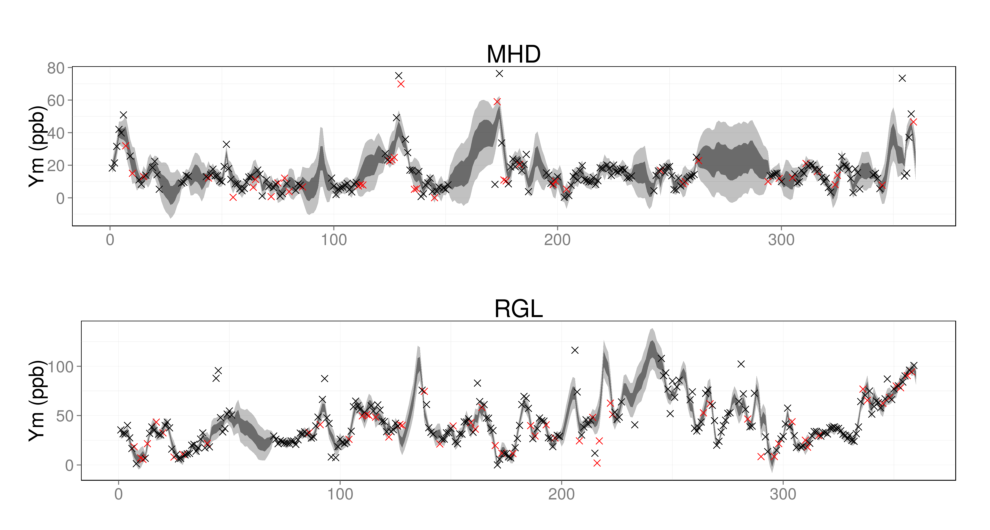
\includegraphics[width=4.3in]{Figure8a.pdf}
	\caption{\footnotesize Distributions of mole fraction due to UK and Ireland land-based emissions at two measurement stations between 1 January 2014 02:00 and 31 January 2014 22:00. The red crosses denote the observations used for validation, whilst the black crosses denote those used for training.}
\end{figure}
\end{center}
\end{frame}



\begin{frame}
\frametitle{Emissions comparison}

\vspace{-0.1in}

\begin{figure}
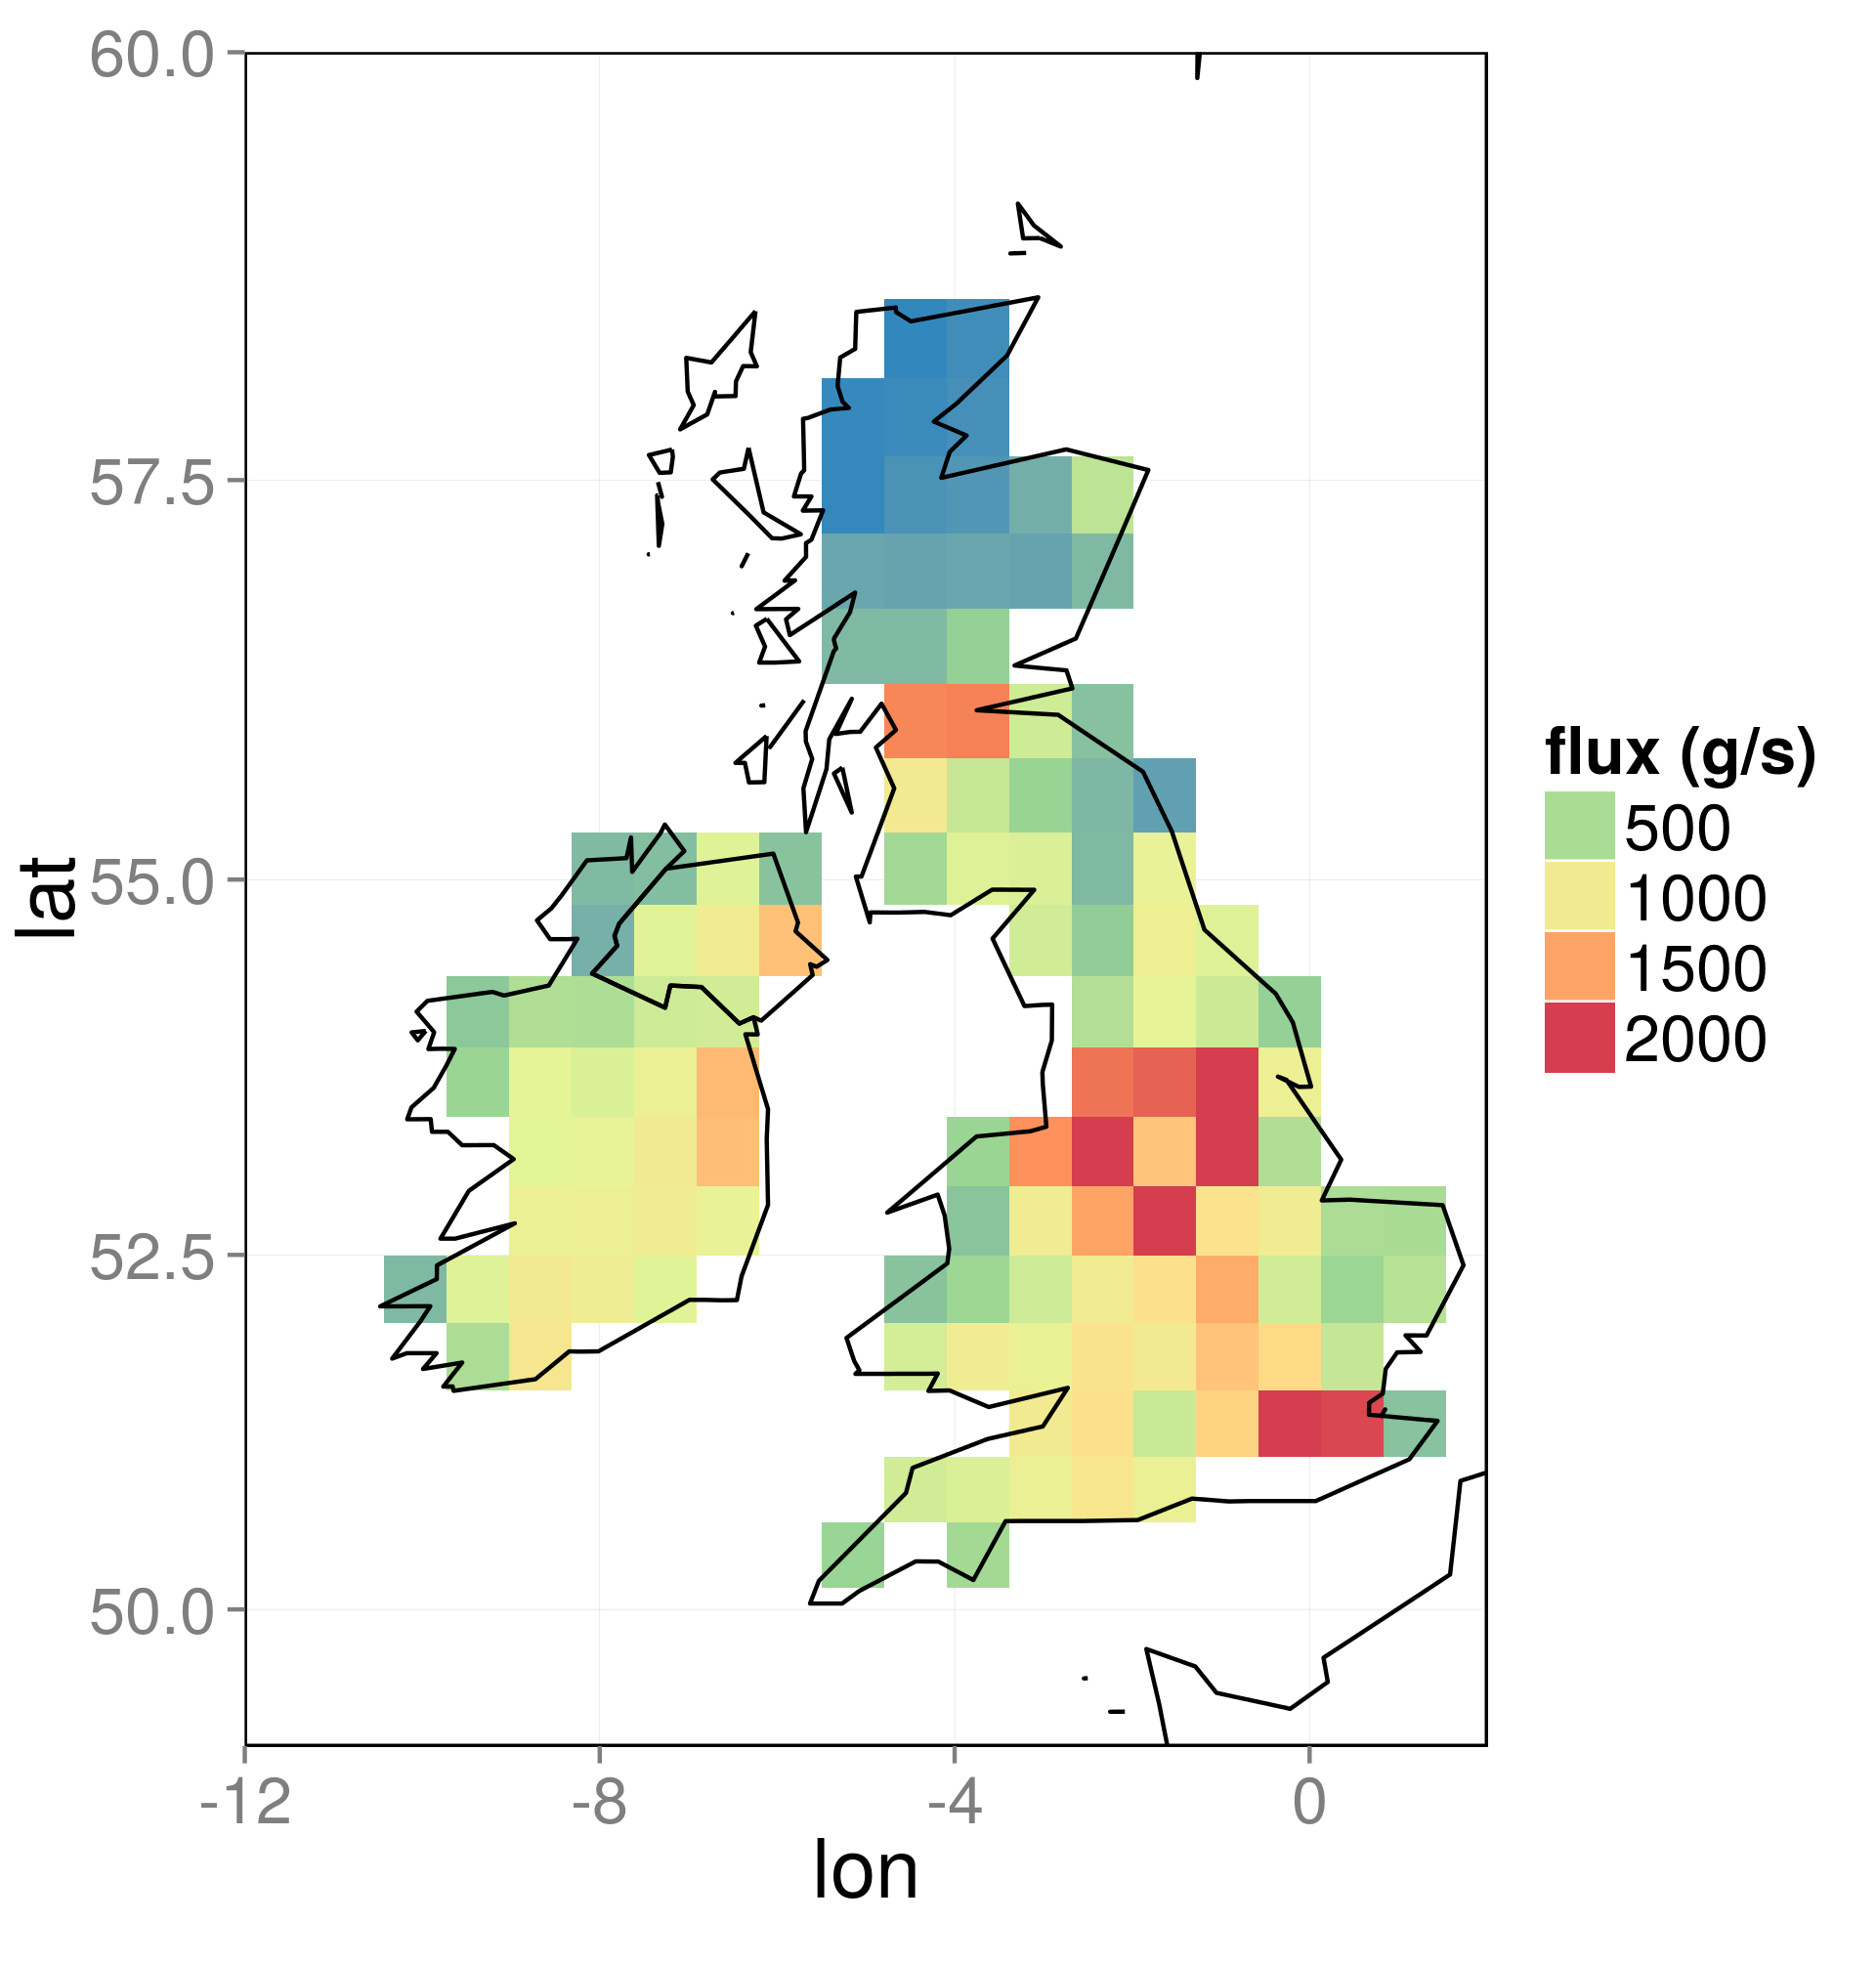
\includegraphics[width=2.0in]{NAEI_land_only.png}
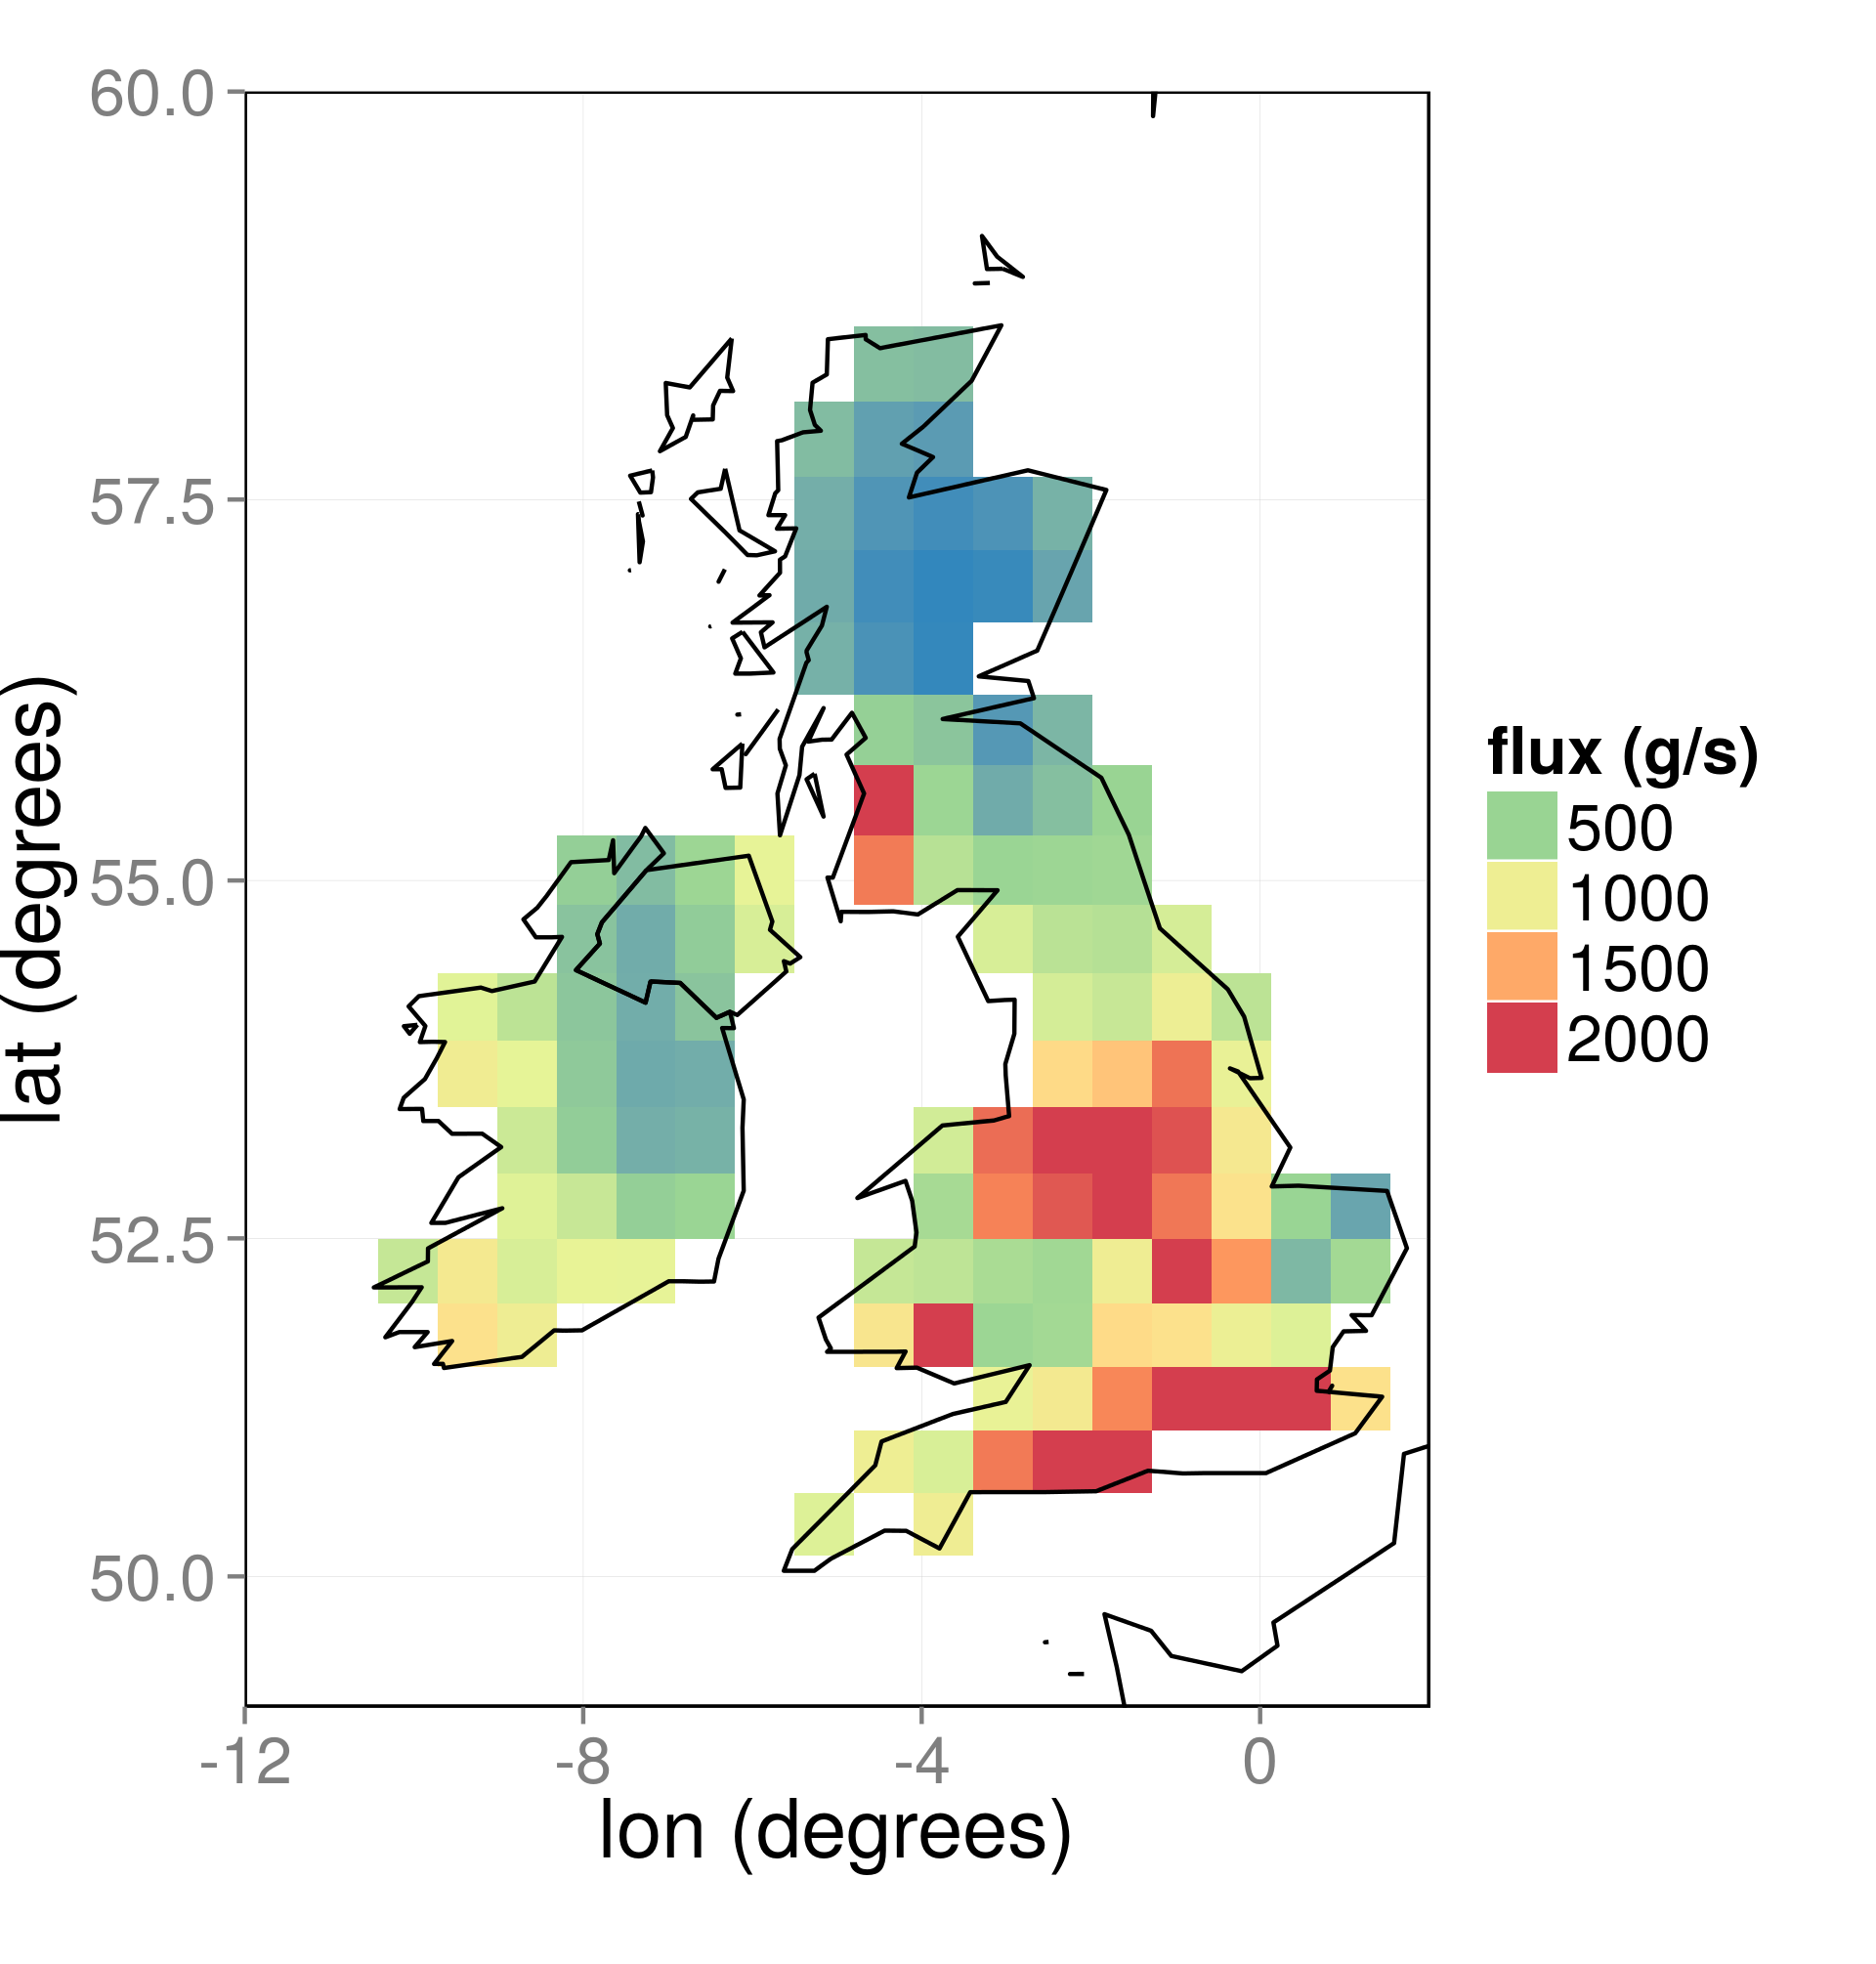
\includegraphics[width=2.0in]{Em95.png}
	\caption{Emissions inventory (left panel) and 95 percentile (right panel) methane emissions in the UK and Ireland, obtained using the Laplace-EM/HMC approach. Emissions in the white grid cells were assumed known and used to correct the observations.}
\end{figure}
\end{frame}



\section{Conclusion}

% \begin{frame}
% \sectionpage
% \end{frame}


\begin{frame}
\frametitle{Conclusions}

\begin{itemize}
\item Bivariate and multivariate models often appear in environmental studies. Usually, one or more of these are `explained away' prior to commencing the analysis. \vfill
\item Such models allow for a (very) flexible model class through interaction functions that can be arbitrarily complex. \vfill
\item Computation is key: For large, non-Gaussian systems, approximate message passing + variational techniques are probably needed \citep{Cseke_2014}. \vfill
\item Slides available from \texttt{https://github.com/andrewzm/bicon}.\vfill
\end{itemize}
\end{frame}

\small

\begin{frame}[allowframebreaks]
\frametitle{References}

\bibliography{../vignettes/Bibliography}


\end{frame}

\end{document}

